\documentclass{sig-alternate}
\usepackage{epsfig}
\usepackage{algorithm}
\usepackage{algorithmic}

 \toappear{
 %\raisebox{2pt}[2pt]{\underline{~~~~~~~~~~~~~~~~~~~~~~~~~~~~~~~~~~~~~~~~~~~~~~~~~~}} \\
 %$^*$ More information on the StreamIt project is available from
 %\texttt{http://compiler.lcs.mit.edu/streamit} \\
   \rule{0cm}{0cm}\\\hrule\rule{0cm}{0cm} ~ \\ \vspace{-6pt} ~ \\
 \parbox[b]{20pc}{\baselineskip 9pt
 Permission to make digital or hard copies of all or part of this work
 for personal or classroom use is granted without fee provided that
 copies are not made or distributed for profit or commercial advantage
 and that copies bear this notice and the full citation on the first
 page.  To copy otherwise, to republish, to post on servers or to
 redistribute to lists, requires prior specific permission and/or a
 fee.} \par
 {\it PLDI'03}, June 9--11, 2003, San Diego, California, USA. \par
 Copyright 2003 ACM 1-58113-662-5/03/0006 ...\$5.00 \\ ~ \\ ~ \\
}

 \conferenceinfo{PLDI'03}{June 9---11, 2003, San Diego, California, USA.}
 \CopyrightYear{2003}
 \crdata{1-58113-662-5/03/0006}

\title{Linear Analysis and Optimization of Stream Programs}
\numberofauthors{1}
\author{
\alignauthor \vspace{-18pt}
Andrew A. Lamb,
William Thies
and Saman Amarasinghe\\
	\vspace{8pt}
	\{aalamb, thies, saman\}@lcs.mit.edu \\
	\vspace{8pt}
	Laboratory for Computer Science \\
	Massachusetts Institute of Technology}


\begin{document}
\newtheorem{definition}{Definition}
\newtheorem{transformation}{Transformation}

\conferenceinfo{PLDI'03,} {June 9--11, 2003, San Diego, California, USA.} 
\CopyrightYear{2003} 
\crdata{1-58113-662-5/03/0006} 

\maketitle

\newcommand{\mt}[1]{\mbox{\it #1}}
\newcommand{\todo}[1]{\framebox{\bf #1}}
\newcommand{\naive}[0]{na\"{\i}ve}
\newcommand{\Naive}[0]{Na\"{\i}ve}
\newcommand{\makeline}[0]{\rule{0cm}{0cm}\\\hrule\rule{0cm}{0cm}}

\begin{abstract}
Due to the high data rates involved in audio, video, and signal
processing applications, it is imperative to compress the data to
decrease the amount of storage used.  Unfortunately, this implies that
any program operating on the data needs to be wrapped by a
decompression and re-compression stage.  Re-compression can incur
significant computational overhead, while decompression swamps the
application with the original volume of data.

In this paper, we present a program transformation that greatly
accelerates the processing of compressible data.  Given a program that
operates on uncompressed data, we output an equivalent program that
operates directly on the compressed format.  Our transformation
applies to stream programs, a restricted but useful class of
applications with regular communication and computation patterns.  Our
formulation is based on LZ77, a lossless compression algorithm
utilized by ZIP, and immediately applies to simpler formats such as
Apple Animation, Microsoft RLE, and Targa.

We implemented a simple subset of our techniques in the StreamIt
compiler, which emits executable plugins for two popular video editing
tools: MEncoder and Blender.  For common operations such as color
adjustment and video compositing, computing directly on compressed
data offers a speedup roughly proportional to the overall compression
ratio.  For our benchmark suite of 12 videos in Apple Animation
format, speedups range from 1.1x to 471x, with a median of 15x.

\end{abstract}

%% Upward of fifty percent of the code that runs the DSP(s) in a modern
%% cell phone is coded in assembly with the rest written in C. Hand
%% optimized assembly code typically makes the best use of the available
%% resources such as power, specialized coprocessors, and specialized
%% instructions.  The problem with assembly code is that the same
%% algorithm must be mapped time and time again whenever a new chip comes
%% out. The life cycle of a typical DSP is much shorter than the life
%% cycle of a general purpose microprocessor -- each new generation is
%% separated by months rather than years.
 
%% Therefore frequently reimplementing algorithms by hand is a costly,
%% arduous process that increases cost and slows the pace of
%% advances. Engineers must spend time working out details rather than
%% focusing on solving harder problems. Compilers were invented forty
%% years ago exactly to let engineers focus on the problem at hand rather
%% than spend time with machine specific details. Compilers for DSP
%% architectures have a difficult job, and are not very good at mapping a
%% program written in a general purpose language like C into the
%% specialized instructions provided by DSPs. Many of the instructions
%% provided by a DSP are targeted for a very specific application (like
%% FIR filtering), but most general purpose languages have no way to
%% describe higher level behavior other than functionally. If you don't
%% express your algorithm in the same way that the compiler expects to
%% encounter it, the resulting program will not take best advantage of
%% the available DSP resources.

\section{Introduction}
Digital computation is becoming an increasingly ubiquitous element of
modern life.  Everything from cell phones to GPS systems to satellite
radios require increasingly sophisticated algorithms.  Optimization is
especially important for this domain, as embedded devices often have
high performance requirements and tight resource constraints.  Even
with the best available C compilers for DSP chips, programmers still
turn to assembly code to implement critical parts of embedded
applications.  This process is time-consuming, error-prone and
costly, and must be repeated for each generation of the target
architecture.  As algorithms and applications continue to grow in
complexity, these factors will become unmanageable.  There is a
pressing need for high-level DSP abstractions that a compiler can
consistently reduce to efficient low-level code.

In this paper, we demonstrate that a domain-specific stream language
can enable novel high-level DSP optimizations that would otherwise be
intractable in a general-purpose language.  Our source language is
StreamIt, which is specifically designed for high-performance signal
processing applications~\cite{streamit-asplos,streamitcc}; our
analysis focuses on filters that are {\it linear}.  StreamIt is
distinguished from a general purpose language in that it makes
explicit the large-scale parallelism and regular communication
patterns that are characteristic of streaming programs.  By analyzing
the primitive building block in StreamIt--the filter--our analysis can
detect large portions of the application that produce outputs as a
linear combination of the inputs; we can exploit this linearity
for a number of large-scale optimizations.  Though each filter is
programmed using imperative C-like code, the separation of filters
into autonomous units of the stream graph enables our analysis to be
far more effective and efficient than it could be on an equivalent
implementation in C alone.

This paper makes the following contributions:
\begin{itemize}

\item A linear dataflow analysis that can extract a linear transfer
function from the imperative code within a StreamIt filter.
\vspace{-6pt}

\item Combination rules for collapsing neighboring linear nodes into a
single linear representation.
\vspace{-6pt}

\item An automated procedure for translating a stream computation into
the frequency domain in order to optimize computationally intensive
linear nodes.
\vspace{-6pt}

\item An implementation of the above techniques in the StreamIt
compiler that automatically improves performance by a factor of
five on average and $6.5$ in the best cast.

\end{itemize}

In the rest of this section, we give a motivating example and
background information on StreamIt.  Then we present our linear
representation (Section~\ref{sec:linearrep}) and our 
supporting dataflow analysis (Section~\ref{sec:dataflow}).  
Next we describe the
combination of linear filters (Section~\ref{sec:combine}) and the
translation to the frequency domain (Section~\ref{sec:freq}) before
giving results (Section~\ref{sec:results}), related work
(Section~\ref{sec:related}), and conclusions
(Section~\ref{sec:conclusion}).

\subsection{Motivating Example}
\begin{figure}[t]
\center
\epsfxsize=2.0in
\epsfbox{images/motivating-example.eps}
\caption{Block diagram of two FIR filters.}
\vspace{11pt}
\scriptsize
\begin{verbatim}
/* perform N-element FIR filter with weights and data */
float filter(float* weights, float* data, int pos, int N) {
  int i;
  float sum = 0;

  /* perform weighted sum, starting at index pos */
  for (i=0; i<N; i++, pos++) {
    sum += weights[i] * data[pos];
    pos = (pos+1)%N;
  }
  return sum;
}

void main() {
  int i;
  float data[N];   /* input data buffer */
  float buffer[N]; /* inter-filter buffer */
  
  /* initialize the input data buffer */
  for (i=0; i<N; i++) {
    data[i] = get_next_input();
  }
  
  /* initialize inter-filter buffer */
  for (i=0; i<N; i++) {
    buffer[i] = filter(weights1, data, i, N);
    data[i] = get_next_input();
  }
  
  i = 0;
  while(true) {
    /* generate next output item */
    push_output(filter(weights2, buffer, i, N));
    /* generate the next element in the inter-filter buffer */
    buffer[i] = filter(weights1, data, i, N);
    /* get next data item */
    data[i] = get_next_input();
    /* update current start of buffer */
    i = (i+1)%N;
  }
}
\end{verbatim}
\vspace{-18pt}
\caption{Two consecutive FIR filters in C.  Channels are represented
as circular buffers, and the scheduling is done by hand.
\protect\label{fig:motivating-example}}
\vspace{-12pt}
\end{figure}

\begin{figure}[t]
\scriptsize
\begin{verbatim}
float->float pipeline TwoPipe {
  add FIRFilter(weights1);
  add FIRFilter(weights2);
}

float->float filter FIRFilter(float[N] weights) {
  work push 1 pop 1 peek N {
    float sum = 0;
    for (int i=0; i<N; i++) {
      sum += weights[i] * peek(i);
    }
    push(sum);
    pop();
}
\end{verbatim}
\vspace{-18pt}
\caption{Two consecutive FIR filters in StreamIt.  Buffer management
and scheduling are handled by the compiler.\protect\label{fig:example-streamit}}
\vspace{6pt}
\begin{verbatim}
float->float filter CollapsedTwoPipe() {
  float[N] combined_weights;

  init {
    /* calculate combined_weights as combination of 
       weights1 and weights2 */
  }

  work push 1 pop 1 peek N {
    float sum = 0;
    for (int i=0; i<N; i++) {
      sum += combined_weights[i]*peek(i);
      }
    push(sum);
    pop();
  }
}
\end{verbatim}
\vspace{-18pt}
\caption{Combined version of the two FIR filters.  Since each FIR
filter is linear, the weights can be combined into a single {\tt
combined\_weights} array.\protect\label{fig:example-combine}}
\vspace{6pt}
%% float->float filter FreqTwoPipe() {
%%   complex[N] H;
%%   init {
%%     H = FFT(combined_weights);
%%   }
%%   work push L pop L peek N+L {
%%     float[N] X = FFT(peek(0..N+L-1)); /* input FFT */
%%     float[N] Y =  X .* H; /* element wise mult */
%%     float[N] y = IFFT(Y); /* inverse FFT */
%%     push(y[0..L-1]); /* push first L elts of y */
%%   }
%% }
\begin{verbatim}
float->float pipeline FreqTwoPipe(int L) {
  float[N] combined_weights = ... ;     // calc. combined weights 
  complex[N] H = fft(combined_weights); // take FFT of weights     
  add FFT(N+L);                         // add FFT stage to stream 
  add ElementMultiply(H);               // add multiplication by H 
  add IFFT(N+L);                        // add inverse FFT         
}
\end{verbatim}
\vspace{-12pt}
\caption{Combined version of two FIR filters in the frequency domain.
\protect\label{fig:example-frequency}}
\vspace{-12pt}
\end{figure}

To illustrate the program transformations that our technique is
designed to automate, consider a sequence of finite impulse response
(FIR) filters as shown in Figure~\ref{fig:motivating-example}. The
imperative C style code that implements this simple DSP application is
also shown. The program largely defies many standard compiler analysis
and optimization techniques because of its use of circular buffers and
the muddled relationship between {\tt data}, {\tt buffer} and the
output.

Figure~\ref{fig:example-streamit} shows the same filtering process
implemented in StreamIt. The StreamIt version is more abstract than
the C version.  It indicates the communication pattern between filters;
it shows the structure of the original block diagram; and it leaves
the complexities of buffer management and scheduling to the compiler.

Two optimized versions of the FIR program are shown in
Figures~\ref{fig:example-combine} and~\ref{fig:example-frequency}.  In
Figure~\ref{fig:example-combine}, the programmer has combined the {\tt
weights} arrays from the two filters into a single, equivalent array.
This reduces the number of multiply operations by a factor of two.  In
Figure~\ref{fig:example-frequency}, the programmer has done the
filtering in the frequency domain, using the FFT and IFFT to translate
between time and frequency.  Computationally intensive filters and
streams are more efficient when done in frequency instead of time.

Our linear analysis can automatically derive both of the
implementations in Figures~\ref{fig:example-combine}
and~\ref{fig:example-frequency}, starting with the code in
Figure~\ref{fig:example-streamit}.  These optimizations free the
programmer from the burden of combining and optimizing linear filters
by hand.  Instead, the programmer can design modular filters at the
natural granularity for the algorithm in question, relying on the
compiler to do the analysis and combination.

\subsection{StreamIt}

%% \begin{figure}
%% \center
%% \epsfxsize=3.0in
%% \epsfbox{images/general-picture-filter.eps}
%% \caption{Graphical illustration of $e_{F}$, $o_{F}$ and $u_{F}$}
%% \label{fig:overview-filter}
%% \end{figure}

StreamIt is a language and compiler for high-performance signal
processing~\cite{gordon-thesis,streamit-asplos,streamitcc}.  In a
streaming application, each data item is in the system for only a
small amount of time, as opposed to scientific applications where the
data set is used extensively over the entire execution.  Also, stream
programs have abundant parallelism and regular communication patterns.
The StreamIt language aims to expose these properties to the compiler
while maintaining a high level of abstraction for the programmer.

StreamIt programs are composed of processing blocks called {\it
filters} which contain an input tape from which they can read values
and an output tape to which they can write. Each filter contains
a {\tt work} function which describes its atomic execution step in the
steady state.  The {\tt work} function contains C-like imperative
code, which can access filter state, call external routines and
produce and consume data.  The input and output channels are treated
as FIFO queues, which can be accessed with three primitive operations:
1) {\tt pop()}, which returns the first item on the input tape and
advances the tape by one item, 2) {\tt peek(i)}, which returns the
value at the $i$th position on the input tape, and 3) {\tt push(v)},
which pushes value {\tt v} onto the output tape.  Each filter
must declare the maximum element it will {\tt peek} at, the number of
elements it will {\tt pop}, and the number of elements that it will
{\tt push} during an execution of {\tt work}.  These rates must be
resolvable at compile time and constant from one invocation of {\tt
work} to the next.  
%Figure~\ref{fig:overview-filter} gives our notation these input/ouput rates.

\begin{figure}[t]
\center
\epsfxsize=3.0in
\epsfbox{images/streamit-structures.eps}
\vspace{-12pt}
\caption{StreamIt structures: {\tt pipeline}, {\tt splitjoin}, and {\tt feedbackloop}.
\protect\label{fig:structures}}
\vspace{-12pt}
\end{figure}

A program in StreamIt consists of a hierarchical graph of {\tt
filters}.  Filters can be connected using one of three predefined
structures (see Figure~\ref{fig:structures}): 1) {\tt pipelines}
represent the serial computation of one filter after another, 2) {\tt
splitjoins} represent explicitly parallel computation, and 3) {\tt
feedbackloops} allow cycles to be introduced into the stream graph.
{\tt filters}, {\tt pipelines}, {\tt splitjoins} and {\tt feedbackloops} are called
{\it streams} and a stream can be used as a subcomponent in a structure.  Note that all {\tt streams} have
exactly one input tape and exactly one output tape.

It has been our experience that most practical applications can be
represented using StreamIt's hierarchical structures.  Though
sometimes a program needs to be reorganized to fit into the structured
paradigm, there are benefits for both the programmer and the compiler
in having a structured language~\cite{streamitcc}.  In particular,
linear analysis relies heavily on the structure of StreamIt to express
stream transformations at a local and hierarchical level.

\section{Filter-Matrix Representations}
In general, a filter take some input and produce some output on
each invocation of its work function. In actual applications, the output
is typically some function of the input and possibly some additional 
filter state. However, there is a large subset of filters in DSP applications
which compute linear functions of the input, which we call ``linear filters.''
If $x[n] n\in[0,peek]$ is the input on each work invocation, then we can 
characterize the output as  $y[k] k\in[0,push] = (\sum_{i=0}^{N} a_{k,i}x[i])+b_{k}$ 
where $w_{n,i}$ is weight of the linear combination of inputs and $C_{k}$ is some
constant value.

As the above equation looks much like the notation for a dot product, 
it is not surprising that we can represent the action of linear filters 
as a vector-matrix product. As figure~\ref{fig:overview-matrix} illustrates, 
to represent a {\tt Filter} $F$'s action as a vector-matrix product, we 
think of the input stream as a row vector $x$ of length $peek_{F}$
and the output as a row vector $y$ of length $push_{F}$. The work function
of $F$ can then be represented as matrix operations using a matrix $A$ and 
a row vector $a$. We can then relate the the input $x$ with the output $y$
with the matrix equation $y$ = $xA + a$. 

$A$ has $peek_{F}$ rows and $push_{F}$ columns, and $a$ has $1$ row 
and $push_{F}$ columns. The elements of $A$ are exactly the weights $a_{k,i}$ 
and the elements of $a$ are exactly the $b_{k}$s.

It is instructive to interpret the matrix of the linear form in the following
way. The columns each represent a formula to compute a specific output, and the 
rows represent the use of a specific input. The rightmost column of $A$ represents
the first output element that is produced (eg the first {\tt push} operation), 
the next rightmost the second output element and so forth. The bottom row 
of $A$ represents the linear combination weight use for the first input 
(eg {\tt peek(0)}), the second to bottom row the second input and so forth.
Using this interpretation to understand what the matrix means helps significantly
in understanding the rationale for the combination rules described later.

\begin{figure}
\center
\epsfxsize=3.0in
\epsfbox{images/general-picture-matrix.eps}
\caption{Linear filter as a vector-matrix operation}
\label{fig:overview-matrix}
\end{figure}

\section{Dataflow Analysis}
The {\tt work} function in each {\tt Filter} can contain arbitrary c-like code, 
and so therefore we ned to run a data analysis pass to determine which filters
are actually computing linear functions of their inputs. The data analysis pass
keeps mappings from variables to linear forms. Linear forms consist of column vectors
of size $peek_{F}$ and a constant.

(need to explain peek/pop/push expressions somewhere.....
 Probably best done with an example)

A linear form can be created in one of three ways. A constant $c$ generates a linear
form with a column vector of zeros and $c$. A {\tt peek(i)} statement generates a linear form
with a column vector with a 1 in the $i^th$ row from the bottom with a zero constant. A
{\tt pop()} expression generates a linear form with a $1$ in the row that is associated with 
the current input element. Of course, there is record keeping to calculate how many {\tt pop}s
a program has performed up to a particular point in the program so that the correct
row can be set to $1$ for {\tt pops} and {\tt peeks}.

Linear forms propagate through the dataflow graph much like constants are propagated
during a standard constant propagation pass. Two linear forms $lf_{1}$ and $lf_{2}$ can
be added together by adding their vectors element wise and adding their constants. Similiarly, 
linear forms can be subtracted. Linear forms can only be multiplied and divided by constants -- if
two linear forms are multiplied together then the result is not a linear combination of the 
filter's input.

If statements are handled just like for constant propagation. The confluence operator that
we use is set intersection, which only propagates variable to linear form mappings that are
maintained along both branches of control flow. We also have to put the restriction that the
same number of pops occured along both branches, or else we don't know what the current offset
for generating peek and pop expressions is. We currently only handle loops that can be unrolled
by a separate unrolling pass in the compiler. A loop can't be unrolled at compile time only if 
its terminiation condition is data dependent. Data dependent loops probably don't compute linear 
functions of the data, and so we declare any variables assigned values in a data dependant loop
to be non linear.

When the {\tt expr} in a {\tt push(expr)} expression is a linear form, we copy its column
vector to the appropriate column in the overall filter's matrix $A$ and we copy the
linear form's constant to the appropriate column in the filter's constant vector $b$.
The first {\tt push} expression places the linear form in the last column of $A$. The second
{\tt push} the second to last column of $A$, etc. The last column of $A$ represents the 
calculations necessary for the first output item produced by the filter. The second to last
column represents the calculatons for the second output item of the filter, etc.

If all the {\tt push} expressions in a filter have linear forms as arguments, then we declare
that the filter is linear and remember the mapping from filter to linear from.

\section{Container Combination(propagation)}
Merely determining that a single filter computes a linear combination of its input is not
all that interesting or useful. There is significant savings to be reaped if we can
find $A$ and $b$ for combinations of filters. Obviously, all of the child filters need
to be linear filters for this combinations to work. We restrict our attention to combining
{\tt Pipelines} and {\tt SplitJoins} because those constructs combine to form a new linear filter. 
{\tt FeedbackLoops} retain state between executions, so the overall construct 
does not compute a linear operation as we have defined it. 

To combine filters, we must deal with rate matching. For instance, if there are two
filters in a pipeline and the first one produces (pushes) 2 elements but the second one
needs 4 elements to produce any output, we need the equivaluet of two firings of the
first filter's {\tt work} function to produce output for the combined filter. 

\begin{figure}
\center
\epsfxsize=3.0in
\epsfbox{images/expanding-a-filter.eps}
\caption{Expanding filter $F$ by a factor $f_{A}$}
\label{fig:expanding-a-filter}
\end{figure}


Therefore, there is a need for a fundamental operation on our representation for 
linear filters to represent producing data from multiple invocations of the work
function. When a linear filter's form is ``expanded'' by a factor $F_{A}$ 
we produce the matrix that describes the output from executing the filter's work
function $f_{A}$ times. Figure~\ref{fig:expanding-a-filter} shows how the {\tt peek},
{\tt pop} and  {\tt push} rates are affected by expanding by factor $f_{A}$.

\begin{figure}
\center
\epsfxsize=3.0in
\epsfbox{images/expanding-a-matrix.eps}
\caption{Expanding a linear form $(A,b)$ by a factor $f_{A}$}
\label{fig:expanding-a-matrix}
\end{figure}

Figure~\ref{fig:expanding-a-matrix} shows the matrix corresponding to expanding 
a filter represented by $(A,b)$ by a factor $f_{A}$. The expansion is done by 
making a new matrix with $f_{A}*push_{F}$ columns and $peek_{F}+(f_{A}-1)*pop_{F}$
rows. The original matrix $A$ is then copied $f_{A}$ times and placed along the
diagonal. Each copy is offset by $push_{F}$ columns and $pop_{F}$ rows.

\subsection{Pipelines}

\begin{figure}
\center
\epsfxsize=3.0in
\epsfbox{images/pipeline-combination.eps}
\caption{Combining a pipeline of two filters.}
\label{fig:combining-pipeline}
\end{figure}

{\tt Pipelines} are serial combinations of filters, one followed directly after 
another. To combine two filters in a pipeline, $F_{1}$ followed by $F_{2}$, we can
simply write down the equations. $F_{1}$ inputs $x$ to prodcue $y_1$ and $F_{2}$
inputs $y_1$ to produce $y_2$. Using our linear filter equations from above,
we can see that $y_1 = xA_1 + b_1$ and $y_2 = y_1A_2 + b_2$. Combining the
two previous equations, it is clear that $y_2 = xA_1A_2 + (A_2b_1 + b_2)$ 
which corresponds to the linear form $(A_1A_2, A_1b_2+b_2)$. 

The above math equations look very simple, but it is not necessairly the case
that you can actually perform the calculation $A_1A_2$ because the dimensions of 
$A_1$ and $A_2$ might not be compatible. For most pairs of linear filters, there
is a choice of scaling factors $f_1$ and $F_2$ that makes the number of columns 
of $A_1$ equal the number of rows of $A_2$.

In general, to make the rates of two filters match, one needs to satisfy
$push_{F_{1}'} = push_{F_{2}'}$ which means that 
$f_1push_{F_1}=peek_{F_2}+(f_2-1)pop_{F_2}$, where $push_{F_1}$,
$peek_{F_2}$ and $pop_{F_2}$ are all arbitrary integers and 
$f_1$ and $f_2$ are integers that must be determined by the compiler.
This constraint is not always satisfiable. For instance if
$push_{F_1}=2$, $peek_{F_2}=3$ and $pop_{F_2}=2$, you can not
choose $f_a$ and $f_2$ to satisfy the above equation.

Figure~\ref{fig:combining-pipeline} shows graphically the process of combining
a pipeline of two filters into a single linear filter.

\subsection{SplitJoins}
{\tt SplitJoins} are the StreamIt construct that allow a programmer to describe explicitly 
parallel computation. Data elements come into the top of the {\tt SplitJoin} and are directed
to the parallel {\tt Filters} by a {\tt Splitter} element. Currently, there are two types of
{\tt Splitters}: a duplicate splitter that merely sends a copy of each data element to each
of the parallel {\tt Filters}. A roundrobin splitter which has $N$ weights, $w_k$ for $k\in[1..N]$
where $N$ is the number of parallel {\tt Filters} in the {\tt SplitJoin}. The first $w_1$ elements
from the input data stream are sent to the leftmost {\tt Filter}. The next $w_2$ elements
are directed to the second leftmost {\tt Filter} and so on. When $sum_{k=0}^{N} w_k$ elements
have been seen, then the pattern starts again from the beginning.

The data from the parallel {\tt Filters} are combined back into a single stream by means of
a roundrobin joiner characterized by weights $v_k$ for $k\in[1..N]$ where $N$ is the number
of parallel streams in the {\tt SplitJoin}. First, $v_1$ items from the leftmost filter
are placed onto the output tape. Then $v_2$ elements from the second leftmost filter are placed
onto the output tape and so on. Again, the process repeats itself after $sum_{k=0}^{N} v_k$
elements have been produced at the output.


\begin{figure}
\center
\epsfxsize=3.0in
\epsfbox{images/splitjoin-combine.eps}
\caption{Combining a {\tt SplitJoin} that is composed of linear streams.}
\label{fig:splitjoin-combine}
\end{figure}

In our linear framework, we can produce a linear representation from any valid {\tt SplitJoin}
given that each of the child streams is linear. If that is the case, then we can describe the
action of the entire {\tt SplitJoin} as a linear operation represented by a new linear form
as shown in Figure~\ref{fig:splitjoin-combine}.

One can think of the joiner of a {\tt SplitJoin} as simply reordering the output data from
the parallel stream blocks. Remembering that each column of a linear form represents the 
formula for calculating a single output of the filter, then it is easy to see the overall form
of a {\tt SplitJoin} is going to consist of a particular order of the columns in the parallel
program streams.

\subsubsection{Duplicate Splitter}

\begin{figure}
\center
\epsfxsize=3.0in
\epsfbox{images/splitjoin-duplicate-ratematch.eps}
\caption{Expanding substreams to match their rates in a {\tt SplitJoin}.}
\label{fig:splitjoin-duplicate-ratematch}
\end{figure}

Combining a {\tt SplitJoin} where the splitter is duplicate is relatively straightforward
since each of the rows in the sub streams refer to the same input items given that the
linear representations of the sub streams have the same number of rows. The same rows in
different linear representations correspond to the same data items because each the 
same data item is copied to each sub stream.

To produce an overall representation by simply ordering the columns of the sub streams'
linear representations, we need to ensure that we could run the joiner
an integer number of times and consume exactly the correct number of items from one
expanded firing from each of the sub streams. To match the output rates we calculate
$x=lcm(\forall k, lcm(push(F_k),w_k))$. One can interpret x as the total number of elements
produced by all of the sub filters. Then we expand each filter $F_i$ by a factor
$f_i=\frac{x}{push(F_i)}$ which means that expanded it will produce $f_i*push(F_i)$ items, and
it will take $f_{w_i}=\frac{x}{w_i}$ firings of the joiner, with each of the firings consuming
$w_i$ elements. It is important to note that in order for the {\tt SplitJoin} to be valid
(eg have a schedule that does not result in an infinite buffer, see \cite{karczma-thesis} for
all of the the gory details) all of the $f_{w_i}$'s must be the same integer.
Figure~\ref{fig:splitjoin-duplicate-ratematch} graphically depicts the process of expanding
the sum linear forms so that the rates are matched. 

\begin{figure}
\center
\epsfxsize=3.0in
\epsfbox{images/splitjoin-duplicate-matrix.eps}
\caption{Matrix resulting from combining a {\tt SplitJoin} with rate matched substreams.}
\label{fig:splitjoin-duplicate-matrix}
\end{figure}

After the rates are matched as described above, we are garenteed to have the same number of rows
in each of the sub streams expanded representations. In order to construct the overall matrix, 
all that remains is to order the columns of the expanded representations appropriately. 
Since we know that the the first $w_1$ output elements will be the first $w_1$ elements 
produced from filter $F_1$ we put the $w_1$ rightmost columns of $A_1$ as the rightmost
columns of the overall representation matrix. We then place the $w_2$ rightmost columns of $A_2$ 
into the next columns of the overall representation matrix, and so forth until
we have determined all of the elements that would have been produced from one firing of 
the joiner ($\sum_{i=0}^{N} w_{i}$). If $f_{w_i}$ is greater than one 
(eg the joiner has to be executed more than once) then we go back and take rightmost
$w_1$ remaining columns from $A_1$, then the rightmost remaining columns from $A_2$, and
so forth. This process repreats until all of the columns from the expanded representations have
been fitted into the overall linear representation. Figure~\ref{fig:splitjoin-duplicate-matrix} 
shows graphically the process of creating the overall matrix.


\subsubsection{Roundrobin Splitter}

\begin{figure}
\center
\epsfxsize=3.0in
\epsfbox{images/splitjoin-roundrobin-to-duplicate.eps}
\caption{Converting a {\tt SplitJoin} with a roundrobin splitter to a {\tt SplitJoin} with a duplicate splitter.}
\label{fig:splitjoin-roundrobin-to-duplicate}
\end{figure}

In some applications, the incoming data to the {\tt SplitJoin} is directed to various sub streams 
by a roundrobin splitter with weights $v_i$. In this case, first we expand the sub streams of the
{\tt SplitJoin} to match the rates as described above and shown in 
Figure~\ref{fig:splitjoin-duplicate-ratematch}. However, after we have expanded, the number of
columns is correct, but the rows of each filter's expanded representation do not represent the
same input elements (because each filter doesn't see data bound to other filters). Therefore,
the matrices aren't necessairly going to have the same number of rows, and so merely
copying columns in the order described above isn't going to work because the columns will be 
of different sizes. To handle the case with a roundrbin splitter, we transform the {\tt SplitJoin} 
into a {\tt SplitJoint} with a duplicate splitter as illustrated in 
Figure~\ref{fig:splitjoin-roundrobin-to-duplicate}. To affect this transformation, we need the rows
of each sub filter's matrix to represent the same data items. By sending all of the data to each filter,
we need to tell each linear representation that its output doesn't depend in any way on the data that 
was originally bound for another filter. We insert rows of $0$s into the expanded representions
for each row that was originally bound for another subfilter. Figure~\ref{fig:splitjoin-roundrobin-matrix}
illustrates how the new matrix is constructed.

\begin{figure}
\center
\epsfxsize=3.0in
\epsfbox{images/splitjoin-roundrobin-matrix.eps}
\caption{Corresponding matrix for splitter conversion from roundrobin to duplicate.}
\label{fig:splitjoin-roundrobin-matrix}
\end{figure}


\newcommand{\la}{$\leftarrow$}
\newcommand{\IND}{\begin{ALC@g}}
\newcommand{\UND}{\end{ALC@g}}
\newcommand{\tup}[2]{\langle{#1}, {#2}\rangle}

\section{Linear Extraction Algorithm}
\label{sec:dataflow}

Our linear extraction algorithm can identify a linear filter and
construct a linear node $\lambda$ that fully captures its behavior.
The technique, which appears as Algorithm~\ref{alg:dataflow} on the
next page, is a flow-sensitive, forward dataflow analysis similar to
constant propagation.  Unlike a standard dataflow analysis, we can
afford to symbolically execute all loop iterations, since most loops
within a filter's work function have small bounds that are known at
compile time (if a bound is statically unresolvable, the filter is
unlikely to be linear and we disregard it).

During symbolic execution, the algorithm computes the following for
each point of the program (refer to Figure~\ref{fig:types} for
notation):
\begin{itemize}

\vspace{-6pt}
\item A $\mt{map}$ between each program variable $y$ and a linear form
$\tup{\vec{v}}{c}$ where $\vec{v}[0 \cdots Peek]$ is a column vector 
and $c$ is a scalar constant. In an actual execution, the value of $y$ would
be given by $y = \vec{v} \cdot \vec{x} + c$, where $\vec{x}$ 
represents the input items.
\vspace{-6pt}

\item Matrix $A$ and vector $\vec b$, which will represent the linear node.
These values are constructed during the operation of the algorithm.
\vspace{-6pt}

\item $\mt{pushcount}$, which indicates how many items have been
pushed so far.  This is used to determine which column of $A$ and
$\vec{b}$ correspond to a given push statement.
\vspace{-6pt}

\item $\mt{popcount}$, which indicates how many items have been popped
so far.  This is used to determine the row in $\vec{v}$ that a 
given peek or pop expression refers to.
\vspace{-6pt}

\end{itemize}

We now briefly discuss the operation of {\bf Extract} at each program
node.  The algorithm is formulated in terms of a simplified set of
instructions, which appear in Figure~\ref{fig:types}.  First are the
nodes that generate fresh linear forms.  A constant assignment $y = c$
creates a form $\tup{\vec 0}{c}$ for $y$, since $y$ has constant part
$c$ and does not yet depend on the input.  A pop operation
creates a form $\tup{\mbox{\bf BuildCoeff}(\mt{popcount})}{0}$, where
{\bf BuildCoeff} introduces a coefficient of $1$ for the current index
on the input stream.  A peek$(i)$ operation is similar, but
offset by the index $i$.

\begin{algorithm}[t]
\caption{Linear extraction analysis.\protect\label{alg:dataflow}}
proc {\bf Toplevel}(filter $F$) returns linear node for $F$ \vspace{-4pt}
\begin{enumerate}
\item Set globals Peek, Pop, Push to I/O rates of filter $F$. \vspace{-4pt}
\item Let $A_{0} \leftarrow \mbox{new float[Peek, Push] with each entry =~} \bot$ \vspace{-14pt}
\item Let ${\vec b_{0}} \leftarrow \mbox{new float[Push] with each entry =~} \bot$ \vspace{-6pt}
\item $(\mt{map}, A, {\vec b}, \mt{popcount}, \mt{pushcount}) \leftarrow$ \\ 
\verb+      +{\bf Extract}$(F_{work}, (\lambda x . \bot), A_{0}, {\vec b_{0}}, 0, 0)$ \vspace{-6pt}
\item {\bf if} $A$ and ${\vec b}$ contain no $\top$ or $\bot$ entries {\bf then} \\
\verb+ + return linear node $\lambda = \{A, {\vec b}, \mbox{Peek}, \mbox{Pop}, \mbox{Push}\}$ \\
 {\bf else} \\
\verb+ + {\it fail} \\
 {\bf endif}
\end{enumerate}
proc {\bf BuildCoeff}(int $pos$) returns $\vec v$ for peek at index $pos$ \\ \vspace{-12pt}
\begin{algorithmic}
\STATE $\vec{v} = \vec{0}$
\STATE $\vec{v}[\mbox{Peek}-1-\mt{pos}] = 1$
\STATE return $\vec{v}$
\end{algorithmic}
\end{algorithm}

\begin{figure}[t]
\vspace{-12pt}
\begin{equation} \nonumber
\begin{array}{rcl}
y & \in & \mbox{program-variable} \\
c & \in & \mbox{constant}^{\top} \\
\vec v, \vec b & \in & \mbox{vector}^{\top} \\
\tup{\vec v}{c} & \in & \mbox{linear-form}^{\top} \\
map & \in & \mbox{program-variable} \rightarrow \mbox{linear-form  (a hashtable)} \\
A & \in & \mbox{matrix}^{\top} \\
code & \in & \mbox{list of instructions, each of which can be:} \\
\multicolumn{3}{l}{\parbox{3in}{
    \vspace{-6pt}
    \begin{equation} \nonumber
      \begin{array}{ll}
	y_1 := \mt{const} & \mbox{{\tt push}}(y_1) \\
	y_1 := \mbox{\tt pop}() & (\mbox{{\tt loop}} ~N~ \mt{code}) \\
        y_1 := \mbox{\tt peek}(i) & (\mbox{{\tt branch}} ~\mt{code}_1~ \mt{code}_2) \\
	y_1 := y_2~\mt{op}~y_3 & ~
      \end{array}
\end{equation}}}
\end{array} 
\end{equation}
\vspace{-18pt}
\caption{Data types for the extraction analysis.\protect\label{fig:types}}
\vspace{-14pt}
\end{figure}

\begin{algorithm}
proc {\bf Extract}($code$, $map$, $A$, $\vec b$, int $\mt{popcount}$, int $\mt{pushcount}$) \\
\verb+   + returns updated $\mt{map}$, $A$, ${\vec b}$, $\mt{popcount}$, and $\mt{pushcount}$ \\ \vspace{-12pt}
\begin{algorithmic}
\FOR {$i \leftarrow 1$ to $\mt{code}$.length}
\STATE {\bf switch} $\mt{code}$[i]
\IND
\STATE $\mbox{\bf case}~y := \mt{const}$
\IND
\STATE $\mt{map}.\mt{put}(y, (\vec 0, \mt{const}))$
\UND
\STATE \vspace{-6pt}
\STATE $\mbox{\bf case}~y := \mbox{\tt pop}()$
\IND
\STATE $\mt{map}.\mt{put}(y, \tup{\mbox{\bf BuildCoeff}(\mt{popcount})}{0})$
\STATE $\mt{popcount}$\verb|++|
\UND
\STATE \vspace{-6pt}
\STATE $\mbox{\bf case}~y := \mbox{\tt peek}(i)$
\IND
\STATE $\mt{map}.\mt{put}(y, \tup{\mbox{\bf BuildCoeff}(\mt{popcount}+i)}{0})$
\UND
\STATE \vspace{-6pt}
\STATE $\mbox{\bf case}~\mbox{\tt push}(y)$
\IND
\STATE $\tup{\vec v}{c} \leftarrow \mt{map}.\mt{get}(y)$
\STATE {\bf if} $\mt{pushcount} = \top$ {\bf then} $\mt{fail}$
\STATE $A[*, \mbox{Push} - 1 - \mt{pushcount}] \leftarrow \vec v$
\STATE $\vec{b}[\mbox{Push} - 1 - \mt{pushcount}] \leftarrow c$
\STATE $\mt{pushcount}$\verb|++|
\UND
\STATE \vspace{-6pt}
\STATE $\mbox{\bf case}~ y_1 := y_2 \mt{~op~} y_3$, for $\mt{~op~} \in \{+, -\}$
\IND
\STATE $\tup{\vec v_2}{c_2} \leftarrow \mt{map}.\mt{get}(y_2)$
\STATE $\tup{\vec v_3}{c_3} \leftarrow \mt{map}.\mt{get}(y_3)$
\STATE $\mt{map}.\mt{put}(y_1, \tup{\vec v_2 \mt{~op~} \vec v_3}{c_2 \mt{~op~} c_3})$
\UND
\STATE \vspace{-6pt}
\STATE $\mbox{\bf case}~y_1 := y_2 * y_3$
\IND
\STATE $\tup{\vec v_2}{c_2} \leftarrow \mt{map}.\mt{get}(y_2)$
\STATE $\tup{\vec v_3}{c_3} \leftarrow \mt{map}.\mt{get}(y_3)$
\STATE {\bf if} $~\vec v_2 = \vec 0$ {\bf then}
\IND
\STATE $\mt{map}.\mt{put}(y_1, (c_2*\vec v_3, c_2*c_3))$
\UND
\STATE {\bf else if} $~\vec v_3=\vec 0$ {\bf then}
\IND
\STATE $\mt{map}.\mt{put}(y_1, (c_3*\vec v_2, c_3*c_2))$
\UND
\STATE {\bf else}
\IND
\STATE $\mt{map}.\mt{put}(y_1, \top)$
\UND
\UND
\STATE \vspace{-6pt}
\STATE $\mbox{\bf case}~y_1 := y_2 / y_3$
\IND
\STATE $\tup{\vec v_2}{c_2} \leftarrow \mt{map}.\mt{get}(y_2)$
\STATE $\tup{\vec v_3}{c_3} \leftarrow \mt{map}.\mt{get}(y_3)$
\STATE {\bf if} $~\vec v_3 = \vec 0 \wedge c_3 \ne 0$ {\bf then}
\IND
\STATE $\mt{map}.\mt{put}(y_1, (\frac{1}{c_3}*\vec v_2, c_2/c_3))$
\UND
\STATE {\bf else}
\IND
\STATE $\mt{map}.\mt{put}(y_1, \top)$
\UND
\UND
\STATE \vspace{-6pt}
\STATE $\mbox{\bf case}~y_1 := y_2 ~\mt{op}~ y_3$, for $\mt{op} \in \{\&, |, \wedge, \&\&, ||, !, \mt{etc.}\}$
\IND
\STATE $\tup{\vec v_2}{c_2} \leftarrow \mt{map}.\mt{get}(y_2)$
\STATE $\tup{\vec v_3}{c_3} \leftarrow \mt{map}.\mt{get}(y_3)$
\STATE $\mt{map}.\mt{put}(y_1, (\vec 0 \sqcup \vec v_2 \sqcup \vec v_3, c_2 ~\mt{op}~ c_3))$
\UND
\STATE \vspace{-6pt}
\STATE \mbox{\bf case}~({\tt loop} N $code'$)
\IND
\STATE \bf{for} $j \leftarrow 1$ to $N$ {\bf do}
\IND
\STATE $(\mt{map}, A, {\vec b}, \mt{popcount}, \mt{pushcount})~\leftarrow~$ \\
\verb+   +\bf{Extract}$(\mt{code}, \mt{map}, A, {\vec b}, \mt{popcount}, \mt{pushcount})$
\UND
\UND
\STATE \vspace{-6pt}
\STATE \mbox{\bf case}~({\tt branch} $code_1~code_2)$
\IND
\STATE $(\mt{map}_1, A_1, {\vec b_1}, \mt{popcount}_1, \mt{pushcount}_1) \leftarrow$ \\
\verb+   +${\mbox{\bf Extract}}(\mt{code}_1, \mt{map}, A, {\vec b}, \mt{popcount}, \mt{pushcount})$
\STATE $(\mt{map}_2, A_2, {\vec b_2}, \mt{popcount}_2, \mt{pushcount}_2) \leftarrow$ \\ 
\verb+   +${\mbox{\bf Extract}}(\mt{code}_2, \mt{map}, A, {\vec b}, \mt{popcount}, \mt{pushcount})$
\STATE $\mt{map} \leftarrow \mt{map}_1 \sqcup \mt{map}_2$
\STATE $A \leftarrow A_1 \sqcup A_2$
\STATE ${\vec b} \leftarrow {\vec b_1} \sqcup {\vec b_2}$
\STATE $\mt{popcount} \leftarrow \mt{popcount}_1 \sqcup \mt{popcount}_2$
\STATE $\mt{pushcount} \leftarrow \mt{pushcount}_1 \sqcup \mt{pushcount}_2$
\UND
\UND %end case
\ENDFOR
\STATE return ($\mt{map}$, $A$, ${\vec b}$, $\mt{popcount}$, $\mt{pushcount}$)
\end{algorithmic}
\end{algorithm}

Next are the instructions which combine linear forms.  In the case of
addition or subtraction, we simply add the components of the linear
forms.  In the case of multiplication, the result is still a linear
form if either of the terms is a known constant ({\it e.g.}
$\vec{v}=\vec{0}$).  For division, the result is linear only if the
divisor is a non-zero constant\footnote{{\small Note that if the
dividend is zero and the divisor has a non-zero coefficients vector,
we cannot conclude that the result is zero, since certain runtime
inputs might cause a singularity.}} and for non-linear operations ({\it
e.g.,} bit-level and boolean), both operands must be known constants.
If any of these conditions are not met, then the LHS is assigned a
value of $\top$, which will mark the filter as non-linear if the value
is ever pushed.

The final set of instructions deal with control flow.  For loops, we
resolve the bounds at compile time and execute the body an appropriate
number of times.  For branches, we have to ensure that all the linear
state is modified consistently on both sides of the branch.  For this
we apply the confluence operator $\sqcup$, which we define for scalar
constants, vectors, matrices, linear forms, and maps.  $c_1 \sqcup
c_2$ is defined according to the lattice constant$^{\top}$.  That is,
$c_1 \sqcup c_2 = c_1$ if and only if $c_1 = c_2$; otherwise, $c_1
\sqcup c_2 = \top$.  For vectors, matrices, and linear forms, $\sqcup$
is defined element-wise; for example, $A' = A_1 \sqcup A_2$ is
equivalent to $A'[i,j] = A_1[i,j] \sqcup A_2[i,j]$.  For maps, the
join is taken on the values: $\mt{map}_1 \sqcup \mt{map}_2$ $=$
$\mt{map'}$, where $\mt{map'}.\mt{get}(x) = \mt{map}_1.\mt{get}(x)
\sqcup \mt{map}_2.\mt{get}(x)$.

Our implementation of linear extraction is also interprocedural.  It
is straightforward to transfer the linear state across a call site,
although we omit this from the pseudocode for the sake of
presentation.  Also implicit in the algorithm description is the fact
that all variables are local to the work function.  If a filter
has persistent state, all accesses to that state are marked as $\top$.

%\section{Dataflow Analysis}
\begin{figure}[t]
\scriptsize
\begin{verbatim}
float->float filter LowPassFilter(float g, float cutoffFreq, int N) {
  float[N] h;

  /* since the impulse response is symmetric, 
   * don't worry about reversing h[n]. */
  init {
    int OFFSET = N/2;
    for (int i=0; i<N; i++) {
      int idx = i + 1;
      // generate real part
      if (idx == OFFSET) 
	/* take care of div by 0 error 
	(lim x->oo of sin(x)/x actually equals 1)*/
	h[i] = g * cutoffFreq / pi; 
      else 
	h[i] = g * sin(cutoffFreq * (idx-OFFSET)) / (pi*(idx-OFFSET));
    }
  }

  /* implement the FIR filtering operation 
   * as the convolution sum. */
  work peek N pop 1 push 1 {
    float sum = 0;
    for (int i=0; i<N; i++) { 
      sum += h[i]*peek(i);
    }
    push(sum);
    pop();
  }
}

\end{verbatim}
\vspace{-12pt}
\caption{\protect\small StreamIt code for a low pass filter.
\protect\label{fig:lowpasscode}}
\vspace{-12pt}
\end{figure}


To understand the dataflow analysis used to extract the linear representation from
a {\tt Filter}'s {\tt work} function, one needs to understand what the code of a 
{\tt work} function contains. Most of the code is arbitrary C-like code that would
be very familiar to a C programmer. There are three function calls that have special 
meaning in a {\tt work} function.

\begin{enumerate}
\item {\tt pop()}: Consumes one data item from the input tape and returns its value.
\item {\tt peek(i)}: Returns the value of the $i$th value on the input tape.
\item {\tt push(v)}: pushes the value of {\tt v} on to the output tape.
\end{enumerate}


Figure~\ref{fig:lowpasscode} contains the code to implement a rectangularly windowed 
low pass filter. Note that the {\tt init} function gets called once when the program
starts up.
 
The central idea of the data analysis pass is very much like constant propagation
except that we keep mappings from variables to linear forms instead of variables to
constants. Linear forms are pairs ($v$, $c$) of column vectors $v$ of size $peek_{F}$ 
and a constant $c$. A linear form represents a formula for computing a value from a
linear combination of the {\tt Filter}'s inputs such that the value of a 
linear form at runtime would be $xv + c$.

A linear form can be created in one of three ways. 
\begin{enumerate}
\item A constant $r$ generates a linear form with $v=0$ and $c=r$. 
\item A {\tt peek(i)} statement generates a linear form with $v$ a column vector of all zeros with 
a one in the $i$th row from the bottom and $c=0$. 
\item A {\tt pop()} expression generates a linear form with a one in the row that is associated with 
the current input element. 
\end{enumerate}

Of course, there is record keeping to calculate how many {\tt pop()}s
the {\tt work} function has performed up to a particular point so that the correct
row can be set to one when we encounter {\tt pop()}s and {\tt peeks(i)}s.

Linear forms propagate through the dataflow graph much like constants are propagated
during a standard constant propagation pass. Two linear forms $l_{1}$ and $l_{2}$ can
be added together by adding their vectors element wise and adding their constants, eg 
$l_1+l_2=(v_1+v_2, c_1+c_2)$. Linear forms can only be multiplied by constants $r$, 
the result of which is simply a scaling of all the elements of $v$ and of $c$ by a factor
$r$. Eg $l*r = (rv,rc)$. If two linear forms are multiplied together 
then the result is not a linear combination of the {\tt Filter}'s input, rather it is
some polynomial function in the input.

{\tt if} statements are handled just like for constant propagation. The confluence operator
is set intersection, which only propagates variable to linear form mappings that are
maintained along both branches of control flow. We also have to impose the special restriction that the
same number of {\tt pops()} occurred along both branches or we don't know what the current offset
for generating linear forms from {\tt peek(i)} and {\tt pop()} expressions is. 
We currently only handle loops that can be unrolled in the 
compiler (eg those loops whose bounds are determinable at compile time). 
A loop can't be unrolled at compile time only if its termination condition is data 
dependent, and data dependent loops probably don't compute linear 
functions of the data anyways.


The final piece of generating a linear representation from a linear form is to 
When the {\tt expr} in a {\tt push(expr)} expression is a linear form $l=(v,c)$, 
we copy $v$ to the appropriate column in the {\tt Filter}'s linear representation matrix $A$ 
and we copy $c$ to the appropriate column in the linear representation's constant vector $a$.
The first {\tt push()} expression places the linear form in the last column of $A$. The second
{\tt push()} the second to last column of $A$, etc. The last column of $A$ represents 
the calculations necessary for the first output item produced by the filter. The second to last
column represents the calculations for the second output item of the filter, etc.
The same positions are chosen for the linear forms' constants in the constant vector $a$.

If all the {\tt push} expressions in a filter have linear forms as arguments, 
then we have determined that the filter is linear and remember the mapping from 
filter to linear representation.

%  could replace ``filter'' by ``stream'' in the next few sentences, but 
% I think it reads better as it is, actually
\section{Combining Linear Filters}
\label{sec:combine}

A primary benefit of linear filter analysis is that neighboring
filters can be collapsed into a single matrix representation if both
of the filters are linear.  This transformation automatically
eliminates redundant computations in linear sections of the stream
graph, thereby allowing the programmer to write simple, modular
filters and leaving the combination to the compiler.  In this section,
we first describe a {\it linear expansion} operation that serves as a
building block for the combination techniques.  We then give rules for
collapsing {\tt pipeline}s and {\tt splitjoin}s into linear nodes; we
do not yet deal with {\tt feedbackloop}s as they require the notion of
``linear state'' which we do not describe here.

\subsection{Linear Expansion}

\begin{figure}[t]
\center
\epsfxsize=3.0in
\epsfbox{images/filter-expand.eps}
\vspace{-6pt}
\caption{Expanding a linear node to rates $(e', o', u')$.  }
\label{fig:expanding-a-matrix}
\vspace{-12pt}
\end{figure}

In StreamIt programs, the input and output rate of each filter in the
stream graph is known at compile time.  The StreamIt compiler
leverages this information to compute a static schedule--that is, an
ordering of the node executions such that each filter will have enough
data available to atomically execute its {\tt work} function, and no
buffer in the stream graph will grow without bound in the steady
state.  A general method for scheduling StreamIt programs is given by
Karczmarek~\cite{karczma-thesis}.

A fundamental aspect of the steady-state schedule is that neighboring
nodes might need to be fired at different frequencies.  For example,
if there are two filters $F_1$ and $F_2$ in a {\tt pipeline} and
$F_1$ produces $2$ elements during its {\tt work} function but $F_2$
consumes $4$ elements, then it is necessary to execute $F_1$ twice for
every execution of $F_2$.

%% \begin{figure}
%% \center
%% \epsfxsize=3.0in
%% \epsfbox{images/expanding-a-filter.eps}
%% \caption{Expanding {\tt stream} $S$ by a factor $f$}
%% \label{fig:expanding-a-filter}
%% \vspace{-12pt}
%% \end{figure}

Consequently, when we combine hierarchical structures into a linear
node, we often need to {\it expand} a matrix representation to
represent multiple executions of the corresponding stream.  This
expansion can be done as follows.

% NOT TRUE ANYMORE
%% If we expand a linear node by a factor of $k$, then one execution of
%% the new node will be exactly equivalent to $k$ executions of the
%% original.

\begin{transformation} (Linear expansion)
% DOUBLE-CHECK whether we're assuming 0-indexed or 1-indexed matrices
Given a linear node $\lambda = \{A, {\vec b}, e, o, u\}$, the expansion of
$\lambda$ to a rate of $(e', o', u')$ is given by $\mbox{\bf
expand}(\lambda, e', o', u') = \{A', {\vec b}', e', o', u'\}$, where
$\mathbf{A'}$ is a $e' \times u'$ matrix and $\mathbf{{\vec b}'}$ is a
$u'$-element row vector:
\vspace{-6pt} \\
\begin{equation} \nonumber
\begin{array}{rcl}
\multicolumn{3}{l}{\mt{shift}(r,c) ~\mt{is a}~ u' \times e' ~\mt{matrix}:} \\
\multicolumn{3}{l}{\parbox{3in}{
    \begin{equation} \nonumber
    \mt{shift}(r,c)[i,j] = \left\{
      \begin{array}{l}
	A[i-r,j-c] \\
	~~~\mt{if}~ i-r \in [0,e-1] \wedge j-c \in [0, u-1] \\
	~ 0 \mt{~otherwise}
      \end{array}
      \right.
    \end{equation}
}} \\ ~ \vspace{-6pt} \\
%
\mathbf{A'} & = & \sum_{m=0}^{\lceil u' / u \rceil} \mt{shift}(u'- u -m*u, e'-e-m*o) \\ ~ \vspace{-4pt} \\
%
\mathbf{{\vec b}'}[j] & = & {\vec b}[u-1-(u'-j-1)~\mt{mod}~u]
%%
%% \raisebox{-14pt}{\parbox{3in}{is created by starting with a zero
%% matrix with $e'$ rows and $u'$ columns.  $A$ is then copied $k$ times
%% along the diagonal. Starting at the top left, each copy of $A$ is
%% offset from the previous copy by $u$ columns and $o$ rows.}} \\ ~ \vspace{-8pt} \\
%% $b'$ & is an row vector containing $k$ adjacent copies of $b$.
\end{array}
\end{equation}
\end{transformation}

The intuition behind linear expansion is straightforward (see
Figure~\ref{fig:expanding-a-matrix}.)  Linear expansion aims to scale
the push, pop, and peek rates of a linear node while preserving the
functional relationship between the values pushed and the values
peeked on a given execution.  To do this, we construct a new matrix
$A'$ that contains copies of $A$ along the diagonal.  To account for
items that are popped between invocations, each copy of $A$ is offset
by $o$ from the previous copy.  The complexity of the definition is
due to the end cases.  If the new push rate $u'$ is not a multiple of
the old push rate $u$, then the last copy of $A$ includes only some of
its columns.  Similarly, if the new peek rate $e'$ exceeds that which
is needed by the diagonal of $A$s, then $A'$ needs to be padded with
zero's at the top (since it peeks at some values without using them in
the computation.)

Note that a sequence of executions of an expanded node $\lambda'$
might not be equivalent to any sequence of executions of the original
node $\lambda$, because expansion resets the push and pop rates and
can thereby modify the ratio between them.  However, if $u' = k * u$
and $o' = k * o$ for some integer $k$, then $\lambda'$ is completely
interchangeable with $\lambda$.  In the combination rules that follow,
we utilize linear expansion both in contexts that do and do not
satisfy this condition.

\subsection{Collapsing Linear Pipelines}

%\begin{figure}
%\center
%\epsfxsize=3.0in
%\epsfbox{images/pipeline-combination.eps}
%\caption{A {\tt pipeline} of two linear forms $(A,b)$ and $(C,d)$ (above) and the same {\tt pipeline} with rate matched forms (below).}
%\label{fig:combining-pipeline}
%\vspace{-12pt}
%\end{figure}

The {\tt pipeline} construct is used to compose streams in sequence,
with the output of stream $i$ connected to the input of stream $i+1$.
The following transformation describes how to collapse two linear
nodes in a {\tt pipeline}; it can be applied repeatedly to collapse
any number of neighboring linear nodes.

\begin{transformation} (Pipeline combination)
Given two linear nodes $\lambda_1$ and $\lambda_2$ where the output of
$\lambda_1$ is connected to the input of $\lambda_2$ in a pipeline
construct, the combination $\mbox{\bf pipe}(\lambda_1, \lambda_2)$ $=$
$\mathbf{ \{A', {\vec b}', e', o', u'\}}$ represents an equivalent node that
can replace the original two.  Its components are as follows:
\begin{equation} \nonumber
\begin{array}{rcl}
\mt{chanPop} & = & \mt{lcm}(u_1, o_2) \\ ~ \vspace{-8pt} \\
\mt{chanPeek} & = & \mt{chanPop} + e_2 - o_2 \\ ~ \vspace{-8pt} \\
\lambda_1^e & = & \mt{expand}(\lambda_1, (\left \lceil \frac{\mt{chanPeek}}{u_1} \right \rceil - 1) * o_1 + e_1, \\
~ & ~ & ~\hspace{0.32in}~ \mt{chanPop} * \frac{o_1}{u_1}, \mt{chanPeek}) \\ ~ \vspace{-8pt} \\
\lambda_2^e & = & \mt{expand}(\lambda_2, \mt{chanPeek}, \\
~ & ~ & ~\hspace{0.32in}~ \mt{chanPop}, \mt{chanPop} * \frac{u_2}{o_2}) \\
\mathbf{A'} & = & A_1^e A_2^e \\ ~ \vspace{-8pt} \\
\mathbf{{\vec b}'} & = & {\vec b}_1^e A_2^e + {\vec b}_2^e \\ ~ \vspace{-8pt} \\
\mathbf{e'} & = & e_1^e \\ ~ \vspace{-8pt} \\
\mathbf{o'} & = & o_1^e \\ ~ \vspace{-8pt} \\
\mathbf{u'} & = & u_2^e
\end{array}
\end{equation}
\end{transformation}

The basic forms of the above equations are simple to derive.  Let
${\vec x}_i$ and ${\vec y}_i$ be the input and output channels, respectively, for
$\lambda_i$.  Then we have by definition that ${\vec y}_1 = {\vec x}_1 A_1 + {\vec b}_1$
and ${\vec y}_2 = {\vec x}_2 A_2 + {\vec b}_2$.  But since $\lambda_1$ is connected to
$\lambda_2$, we have that ${\vec x}_2 = {\vec y}_1$ and thus 
${\vec y}_2 = {\vec y}_1 A_2 + {\vec b}_2$.
Substituting the value of ${\vec y}_1$ from our first equation gives ${\vec y}_2 =
{\vec x}_1 A_1 A_2 + {\vec b}_1 A_2 + {\vec b}_2$.  Thus, the intuition is that the
two-filter sequence can be represented by matrices $A' = A_1 A_2$
and ${\vec b}' = {\vec b}_1 A_2 + {\vec b}_2$, with peek and pop rates borrowed from
$\lambda_1$ and the push rate borrowed from $\lambda_2$.

However, there are two implicit assumptions in the above analysis
which complicate the equations for the general case.  First, the
dimensions of $A_1$ and $A_2$ must match for the matrix multiplication
to be well-defined.  If $u_1 \ne e_2$, this will require constructing
expanded nodes $\lambda_1^e$ and $\lambda_2^e$ in which the push and
peek rates match (and thus $A_1^e$ and $A_2^e$ can be multiplied.)

The second complication is with regards to peeking.  If the downstream
node $\lambda_2$ peeks at items which it does not consume ({\it i.e.},
if $e_2 > o_2$), then there needs to be a buffer to hold items that
are read during multiple invocations of $\lambda_2$.  However, in our
current formulation, a linear node has no concept of internal state,
such that this buffer cannot be incorporated into the collapsed
representation.  To deal with this issue, we adjust the expanded form
of $\lambda_1$ to recalculate items that $\lambda_2$ uses more than
once, thereby trading computation for storage space.  This adjustment
is evident in the push and pop rates chosen for $\lambda_1^e$: though
$\lambda_1$ pushes $u_1$ items for every $o_1$ items that it pops,
$\lambda_1^e$ pushes $\mt{chanPeek}*u_1$ for every $\mt{chanPop}*o_1$
that it pops.  When $\mt{chanPeek}>\mt{chanPop}$, this means that the
outputs of $\lambda_1^e$ are overlapping, and
$\mt{chanPeek}-\mt{chanPop}$ items are being regenerated on every
firing.

Note that although $\lambda_1^e$ performs duplicate computations in
the case where $\lambda_2$ is peeking, this computation cost can be
amortized by increasing the value of $\mt{chanPop}$.  That is, though
the equations set $\mt{chanPop}$ as the {\it least} common multiple of
$u_1$ and $o_2$, any common multiple is legal.  As $\mt{chanPop}$
grows, the regenerated portion $\mt{chanPeek}-\mt{chanPop}$ becomes
smaller on a percentage basis.

However, it is the case that some collapsed linear nodes are always
less efficient than the original pipeline sequence.  The worst case is
when $A_1^e$ is a column vector and $A_2^e$ is a row vector, which
requires $O(N)$ operations originally but $O(N^2)$ operations if
combined (assuming vectors of length $N$).  In general, the
compiler can identify performance-degrading combinations when the
number of non-zero elements in $A'$ exceeds the sum of non-zero
elements in $A_1^e$ and $A_2^e$.
% ARE WE SURE THAT LAST SENTENCE IS TRUE?  I think it's more complicated 
% when the pop/peek rate is varied, etc.
% I think that we can -- it just isn't implemented. We have to 
% take a global view of the computation being performed.

\subsection{Collapsing Linear SplitJoins}

The {\tt splitjoin} construct allows the StreamIt programmer to
express explicitly parallel computations.  Data elements that arrive
at the {\tt splitjoin} are directed to the parallel child streams
using one of two pre-defined {\tt splitter} constructs: 1) duplicate,
which sends a copy of each data item to all of the child streams, and
2) roundrobin, which distributes items cyclically according to an
array of weights.  The data from the parallel streams are
combined back into a single stream by means of a roundrobin {\tt
joiner} with an array of weights $w$.  First, $w_0$ items from the
output tape of the leftmost child are placed onto the overall output
tape, then $w_1$ elements are taken from the second leftmost child,
and so on.  The process repeats itself after one complete set of
$\sum_{i=0}^{N-1} w_i$ elements has been pushed.

In this section, we demonstrate how to collapse a {\tt splitjoin} into
a single linear node when all of its children are linear nodes.  Since
the children of {\tt splitjoin}s in StreamIt can be parameterized, it
is often the case that all sibling streams are linear if any one of
them is linear.  However, if a {\tt splitjoin} contains only a few
adjacent streams that are linear, then these streams can be combined
by wrapping them in a hierarchical splitjoin and then collapsing the
wrapper completely.  Our technique also assumes that each 
{\tt splitjoin} admits a valid steady-state schedule; this property is
verified by the StreamIt semantic checker.

\begin{figure}[t]
\center
\epsfxsize=3.0in
\epsfbox{images/splitjoin-combination.eps}
\caption{Matrix resulting from combining a {\tt splitjoin} of rate matched sub streams.
\protect\label{fig:splitjoin-duplicate-matrix}}
\vspace{-12pt}
\end{figure}

Our analysis distinguishes between two cases.  For duplicate
splitters, we directly construct a linear node from the child streams.
For roundrobin splitters, we translate the {\tt splitjoin} to use a
duplicate splitter and then rely on the first analysis to construct a
linear node.  We describe these translations below.

\subsubsection{Duplicate Splitter}

Intuitively, there are three main steps to combining a duplicate
splitjoin into a linear node.  Since the combined node will represent
a steady-state execution of the splitjoin construct, we first need to
expand each child node according to its multiplicity in the schedule.
Secondly, we need to ensure that each child's matrix representation
has the same number of rows--that is, that each child peeks at the
same number of items.  Once these conditions are satisfied, we can
construct a matrix representation for the splitjoin by simply
arranging the columns from child streams in the order specified by the
roundrobin joiner (see Figure~\ref{fig:splitjoin-duplicate-matrix}).
This third step is simplified by the fact that, with a duplicate
splitter, each row of a child's linear representation refers to the
same input element to the splitjoin.

The following transformation describes splitjoin combination in
mathematical terms.

%\begin{figure}
%\center
%\epsfxsize=3.0in
%\epsfbox{images/splitjoin-duplicate-ratematch.eps}
%\caption{Expanding sub {\tt streams} to match their output rates in a linear {\tt SplitJoin}.}
%\label{fig:splitjoin-duplicate-ratematch}
%\end{figure}

\begin{transformation} (Duplicate splitjoin combination)
Given a splitjoin $s$ containing a duplicate splitter, children that
are linear nodes $\lambda_0 \dots \lambda_{n-1}$, and a roundrobin
joiner with weights $w_0 \dots w_{n-1}$, the combination $\mbox{\bf
splitjoin}(s)$ $=$ $\mathbf{ \{A',}$ $\mathbf{{\vec b}',}$ $\mathbf{e',}$
$\mathbf{o',}$ $\mathbf{u'\}}$ represents an equivalent node that can
replace the entire stream $s$.  Its components are as follows:
\begin{equation} \nonumber
\begin{array}{rcl}
\mt{joinRep} & = & \mt{lcm}(\frac{\mt{lcm}(u_0,w_0)}{w_0}, \dots, \frac{\mt{lcm}(u_{n-1},w_{n-1})}{w_{n-1}}) \\
\mt{maxPeek} & = & \mt{max}_i (o_i * \mt{rep}_i + e_i - o_i) \\ ~ \vspace{-2pt} \\
\multicolumn{3}{l}{\forall k \in [0, n-1]:} \\ ~ \vspace{-6pt} \\
\mt{wSum}_k & = & \sum_{i=0}^{k-1} w_i \\ ~ \vspace{-6pt} \\
\mt{rep}_k & = & \frac{w_k * \mt{joinRep}}{u_k} \\ ~ \vspace{-6pt} \\
\lambda_k^e & = & \mt{expand}(\lambda_k, \mt{maxPeek}, 
                              o_k * \mt{rep}_k, u_k * \mt{rep}_k) \\ ~ \vspace{-2pt} \\
\multicolumn{3}{l}{\forall k \in [0, n-1], \forall m \in [0, joinRep-1], \forall n \in [0, u_k-1]:} \\ ~ \vspace{-6pt} \\
\multicolumn{3}{l}{\mathbf{A'}[*, u'-1-n - m * \mt{wSum}_{n}-\mt{wSum}_{k}] = 
  A_{k}^e [*,u_k^e-1-n]} \\ ~ \vspace{-6pt} \\
\multicolumn{3}{l}{\mathbf{{\vec b}'}[u'-1-n - m * \mt{wSum}_{n}-\mt{wSum}_{k}] = 
  b_{k}^e [u_k^e-1-n]} \\ ~ \vspace{-2pt} \\
\mathbf{e'} & = & e_0^e = \dots = e_{n-1}^e \\
\mathbf{o'} & = & o_0^e = \dots = o_{n-1}^e \\
\mathbf{u'} & = & \mt{joinRep} * \mt{wSum}_n \\
\end{array}
\end{equation}
\end{transformation}

The above formulation is derived as follows.  The $\mt{joinRep}$
variable represents how many cycles the joiner completes in an
execution of the splitjoin's steady-state schedule; $\mt{joinRep}$ is
the minimal number of cycles required for each child node to execute
an integral number of times and for all of their output to be consumed
by the joiner.  Similarly, $\mt{rep}_k$ gives the execution count for
child $k$ in the steady state.  Then, in keeping with the procedure
described above, $\lambda_k^e$ is the expansion of the $k$'th node by
a factor of $\mt{rep}_k$, with the peek value set to the maximum peek
across all of the expanded children.  Following the expansion, each
$\lambda_i^e$ has the same number of rows, as the peek uniformization
caused shorter matrices to be padded with rows of zero's at the top.

The final phase of the transformation is to re-arrange the columns of
the child matrices into the columns of $A'$ and ${\vec b}'$.
Figure~\ref{fig:splitjoin-duplicate-matrix} elucidates this process,
though its notation is somewhat cumbersome.  The equation can be
understood as follows: for the $k$'th child and the $m$'th cycle of
the joiner, the $n$'th item that is pushed by child $k$ will
appear at a certain location on the joiner's output tape.  This
location (relative to the start of the node's execution) is $n + m *
\mt{wSum}_n + \mt{wSum}_k$, as the reader can verify.  But since the
right-most column of each array $A$ holds the first item to be pushed,
we need to subtract this location from the width of $A$ when we are
re-arranging the columns.  The width of $A$ is the total number of
items pushed--$u'$ in the case of $A'$ and $u_k^e$ in the case of
$A_k^e$.  Hence the equation as written above: we copy all items in a
given column from $A_k^e$ to $A'$, defining each location in $A'$
exactly once.  The procedure for $b$ is analogous.

Finally, it remains to calculate the peek, pop, and push rates of the
combined node.  The peek rate $e'$ is simply $maxPeek$, which we
defined to be equivalent for all the expanded child nodes.  The push
rate $\mt{joinRep}*\mt{wSum}_m$ is equivalent to the number of items
processed through the joiner in one steady-state execution.  Finally,
for the pop rate we rely on the fact that the splitjoin is well-formed
and admits a schedule in which no buffer grows without bound.  If this
is the case, then the $\mt{pop}$ rates must be equivalent for all the
expanded streams; otherwise, some outputs of the splitter would
accumulate infinitely on the input channel of some stream.  

These input and output rates--in combination with the values of $A'$
and ${\vec b}'$ defined above--define a linear node that exactly represents
the parallel combination of child nodes that are fed by a duplicate
splitter.

\subsubsection{Roundrobin Splitter}

In the case of a roundrobin splitter, items are directed to each child
stream $s_i$ according to weight $v_i$: the first $v_0$ items are sent
to $s_0$, the next $v_1$ items are sent to $s_1$, and so on.  Since a
child never sees the items that are sent to sibling streams, the items
that are seen by a given child form a periodic but non-contiguous
segment of the splitjoin's input tape.  Thus, in collapsing the
splitjoin, we are unable to directly use the columns of child matrices
as we did with a duplicate splitter, since with a roundrobin splitter
these matrices are operating on disjoint sections of the input.

Instead, we collapse linear splitjoins with a roundrobin splitter by
converting the splitjoin to use a duplicate splitter.  In order to
maintain correctness, this involves adding a decimator on each branch
of the splitjoin that eliminates items which were intended for other
streams.

\begin{transformation} (Roundrobin to duplicate)
Given a splitjoin $s$ containing a roundrobin splitter with weights
$v_0 \dots$ $v_{n-1}$, children that are linear nodes $\lambda_0 \dots
\lambda_{n-1}$, and a round-robin joiner $j$, the transformed
$\mbox{\bf rr-to-dup}(s)$ is a splitjoin with a duplicate splitter,
linear child nodes $\mathbf{\lambda_0'} \dots
\mathbf{\lambda_{n-1}'}$, and roundrobin joiner $j$.  The child nodes
are computed as follows:
\begin{equation} \nonumber
\begin{array}{rcl}
\mt{vSum}_k & = & \sum_{i=0}^{k-1} v_i \\ ~ \vspace{-6pt} \\
\mt{vTot} & = & \mt{vSum}_n \\ ~ \vspace{-4pt} \\
\multicolumn{3}{l}{\forall k \in [0, n-1]:} \\ ~ \vspace{-12pt} \\ 
\multicolumn{3}{l}{\parbox{3in}{
    \begin{equation} \nonumber
      \begin{array}{l}
      ~~~~\mt{decimate}[k] ~\mt{is a linear node}~ \{A, \vec 0, \mt{vTot}, \mt{vTot}, \mt{vTot}\} \\
	~~~~~~~\mt{where}~A[i,j] = \left\{
	\begin{array}{l}
	  1 ~\mt{if}~ i=j ~\wedge~ \\ 
	  ~\hspace{0.13in}~ vTot-vSum_{k+1} \le i ~\wedge~ \\
	  ~\hspace{0.13in}~ i < vTot-vSum_{k} \\
	  0 ~\mt{otherwise}
	\end{array}
	\right.
      \end{array}
    \end{equation}}} \\
\mathbf{\lambda_k'} & = & \mt{pipe}(\mt{decimate}[k], \lambda_k)
\end{array}
\end{equation}
\end{transformation}

In the above translation, we utilize the linear pipeline combinator
$\mt{pipe}$ to construct each new child node $\lambda_i^e$ as a
composition of a decimator and the original node $\lambda_i$.  Each
decimator is a square matrix that produces and consumes $\mt{vTot}$
items, which is the number of items processed in one cycle of the
roundrobin joiner.  Those items intended for stream $i$ are copied
with a coefficient of $1$, while all others are eliminated with a
coefficient of $0$.

%% \begin{figure}
%% \center
%% \epsfxsize=3.0in
%% \epsfbox{images/splitjoin-roundrobin-matrix.eps}
%% \caption{Corresponding matrix for splitter conversion from roundrobin to duplicate.}
%% \label{fig:splitjoin-roundrobin-matrix}
%% \end{figure}

\subsection{Applications of Linear Combination}

%% Linear analysis is valuable because it provides a precise relationship
%% between input and output that is nearly impossible to extract from
%% general-purpose imperative programs.  While the combination of linear
%% structures is analogous to algebraic simplification between loop
%% bodies in an imperative program, it would be extremely difficult for a
%% general-purpose compiler to extract the same information.

%% Combining the action of {\tt streams} in a {\tt pipeline} is analogous
%% to algebraic simplification between the bodies of sequential loops in
%% an imperative program.  Once an overall linear node for the {\tt
%% pipeline} has been determined, our compiler can perform this
%% transformation automatically, leaving the the programmer to express
%% the computation in the most convenient manner.

There are numerous instances where the linear combination
transformation could benefit a programmer.  For example, although a
bandpass filter can be implemented with a low pass filter followed by
a high pass filter, actual implementations tend to determine the
coefficients of a single combined filter that performs the same
computation. While a simple bandpass filter is easy to combine
manually, in an actual system several different filters might be
designed and implemented by several different engineers, making 
overall filter combination infeasible.

Another common operation in discrete time signal processing is
downsampling to reduce the computational requirements of a system.
Downsampling is most often implemented as a low pass filter followed
by an $M$ compressor which passes every $M$th input sample to the
output.  In practice, the filters are combined to avoid computing dead
items in the low pass filter.  However, the system specification
contains both filters for the sake of understanding.  Our analysis can
start with the specification and derive the efficient version automatically.

A final example is a multi-band equalizer, in which $N$ different
frequency bands are filtered in parallel (see our FMRadio benchmark).
If these filters are time invariant, then they can be collapsed into a
single node.  However, designing this single overall filter is
difficult, and any subsequent changes to any one of the sub filters
will necessitate a total redesign of the filter.  With our automated
combination process, any subsequent design changes will necessitate
only a recompile rather than a manual redesign.

\section{Translation to Frequency}
\label{sec:freq}

In this section, we demonstrate how we can leverage our linear
representation to automatically perform a common domain-specific
optimization: translation to the frequency domain.  First, we show
that a linear node is equivalent to a set of convolution sums, which
can benefit from algorithmic gains if performed in frequency rather
than time.  We then present an optimized code generation strategy for
transforming linear nodes to frequency.

\subsection{Basic Frequency Implementation}

Our first goal is to show that the computation of a linear node can be
represented as a convolution sum.  Consider executing $m$ iterations
of a linear node $\lambda = \{A, {\vec 0}, e, 1, 1\}$---that is, a
node with $\vec{b} = 0$ and $\mbox{push}=\mbox{pop}=1$ (these assumptions
will be relaxed below).  Let $\vec{out}[i]$ represent the $i$th value
that is pushed during execution, let $\vec{in}[i]$ hold the value of
$peek(i)$ as seen before the execution begins, and let ${\vec y}$ be
the convolution of the only column of $A$ with the vector $\vec{in}$
(that is, $y = A[*,0] * {\vec{in}}$).  Note that $\vec{out}$ is an
$m$-element vector, $A[*,0]$ is an $e$-element vector, ${\vec{in}}$ is
an $(m+e-1)$-element vector, and ${\vec y}$ is an $(m+2e-2)$-element
vector.

Then, we make the following claim:
\begin{equation}
\label{eq:claim1}
\forall i \in [0, m-1]:~~{\vec{out}}[i] = {\vec y}\hspace{1pt}[i+e-1]
\end{equation}
To see that this is true, recall the definition of convolution:
\[
  {\vec y}\hspace{1pt}[i] = A[i,0] * \vec{in}[i] = \sum_{k=-\infty}^{\infty} A[k,0] \vec{in}[i-k]
\]
Substituting $\vec{in}$ by its definition, and restricting $k$ to
range over the valid rows of $A$, we have:
\[
  {\vec y}\hspace{1pt}[i] = \sum_{k=0}^{e-1} A[k,0] \mbox{peek}(i-k)
\]
Remapping the index $i$ to $i+e-1$ makes the right hand side
equivalent to ${\vec{out}}[i]$, by Definition 1.
Claim~\ref{eq:claim1} follows.

In other words, values pushed by a linear node can be calculated by a
convolution of the input tape with the coefficients $A$.  The
significance of this fact is that a convolution operation can be
implemented very efficiently by using the Fast Fourier Transform (FFT)
to translate into the frequency domain.  To compute the convolution,
two $N$-point FFTs of $\vec{in}$ and $A[*,0]$ are calculated to obtain
$\vec{X}$ and $\vec{\cal A}$, each of which is a complex-valued vector
of length $N$.  Element-wise multiplication of $\vec X$ and
$\vec{\cal A}$ yields a vector $\vec{Y}$, to which the inverse
transform (IFFT) is applied to obtain $\vec{y}$.  Convolution in the
frequency domain requires $O(N \lg(N))$ operations, as each FFT and
IFFT has a cost of $O(N \lg (N))$ and the vector multiplication is
$O(N)$.  By contrast, the complexity is $O(N^2)$ in the time domain,
as each of the $N$ output values requires $O(N)$ operations.  For more
details, refer to~\cite{oppenheim-discrete}.

We can use the procedure described above to implement a linear node in
the frequency domain.  We simply calculate ${\vec y} = A[*,0] * {\vec
in}$, and extract values ${\vec y}\hspace{1pt}[e-1] \dots {\vec y}\hspace{1pt}[m+(e-1)-1]$ as
the $m$ values pushed by the node.  Note that ${\vec y}\hspace{1pt}[i]$ is also
defined for $i \in [0, e-2]$ and $i \in [m+e-1,m+2e-2]$; these values
represent partial sums in which some coefficients were excluded.  Our
{\naive} implementation simply disregards these values.  However, in the
next section, we give an optimized implementation that takes advantage
of them.

The only task remaining for the implementation is to choose $N$, the
FFT size, and $m$, the number of iterations to execute at once in the
frequency domain.  According to Fourier's theorem, an $N$-point FFT
can exactly represent any discrete sequence of $N$ numbers, so the
only constraint on $N$ and $m$ is that $N \ge m+2e-1$.  For
performance reasons, $N$ should be a power of two and as large as
possible.  In our implementation, we set $N$ to the first power of two
that is larger than $2e$, which strikes a reasonable compromise
between storage space and performance for our uniprocessor
benchmarking platform.  The choice of $N$ should be adjusted for the
particular resource constraints of the target architecture.

The transformation below gives a {\naive} translation of a linear node to
the frequency domain.  In addition, it relaxes all of the assumptions
that we made above.  The algorithm allows for a non-zero value of
${\vec b}$ by simply adding $\vec{b}$ after returning from the
frequency domain.  To accommodate a push rate greater than one, the
algorithm generates $\vec{Y}$ and $\vec{y}$ {\it matrices} and
alternates pushing values from each column of $\vec{y}$ in turn.
Finally, to accommodate a pop rate greater than one, the algorithm
proceeds as if the pop rate was one and adds a special decimator node
that discards the extra outputs.  Though this introduces inefficiency
by calculating values that are never used, it still leaves room for
large performance improvements, as the frequency transformation
improves performance by an average factor of 50 (in the case where
$\mbox{pop}=1$.)

\begin{transformation} ({\Naive} frequency implementation)
Given a linear node $\lambda = \{A, {\vec b}, e, o, u\}$, the
following stream is a {\naive} implementation of $\lambda$ in the
frequency domain:
\begin{equation} \nonumber
{\small
  \begin{array}{ll}
    {\tt float \rightarrow float}~{\tt pipeline~naiveFreq~}(A, {\vec b}, e, o, u){\tt ~\{} & \hspace{40pt}\\
    ~~{\tt add~float \rightarrow float~filter~\{}\\
    ~~~~N \leftarrow 2^{\lceil \lg(2e) \rceil} \\
    ~~~~m \leftarrow N-2e+1 \\
    \\
    ~~~~{\tt init}~{\tt \{} \\
    ~~~~~~{\tt for}~j=0~{\tt to}~u-1\\
    ~~~~~~~~\vec{H}[*,j] \leftarrow \mathbf{FFT}(N,A[*,u-1-j]) \\
    ~~~~{\tt \}} \\
    \\
    ~~~~{\tt work}~{\tt peek}~m+e-1~{\tt pop}~m~{\tt push}~u*m~{\tt \{} \\
    ~~~~~~\vec{x} \leftarrow {\tt peek}(0 \dots m+e-1 ) \\
    ~~~~~~\vec{X} \leftarrow \mathbf{FFT} (N, \vec{x}) \\
    ~~~~~~{\tt for}~j=0~{\tt to}~u-1\\
    ~~~~~~~~\vec{Y}[*,j] \leftarrow \vec{X} .* \vec{H}[*,j] \\
    ~~~~~~~~\vec{y}\hspace{1pt}[*,j] \leftarrow \mathbf{IFFT}(N, \vec{Y}[*,j]) \\
    ~~~~~~{\tt \}} \\
    ~~~~~~{\tt for}~i=0~{\tt to}~m-1\\
    ~~~~~~~~{\tt pop()} \\
    ~~~~~~~~{\tt for}~j=0~{\tt to}~u-1\\
    ~~~~~~~~~~{\tt push}(\vec{y}\hspace{1pt}[i+e-1,j] + {\vec b}[j])\\
    ~~~~~~{\tt \}} \\
    ~~~~{\tt \}} \\
    ~~{\tt \}} \\
    ~~{\tt add~FreqDecimator(o, u)} \\
    {\tt \}} \\ ~ \\
    {\tt float \rightarrow float}~{\tt filter~freqDecimator~}(o, u){\tt ~\{} & \hspace{40pt}\\
    ~~{\tt work~}{\tt peek}~u*o~{\tt pop}~u*o~{\tt push}~u~{\tt \{} \\
    ~~~~{\tt for}~i=0~{\tt to}~u-1 \\
    ~~~~~~{\tt push(pop())} \\
    ~~~~{\tt for}~i=0~{\tt to}~u-1 \\
    ~~~~~~{\tt for}~j=0~{\tt to}~o-2 \\
    ~~~~~~~~{\tt pop()} \\
    ~~{\tt \}} \\
    {\tt \}}
  \end{array}}
\end{equation}
\vspace{-6pt}
\label{trans:freq1}
\end{transformation}

\subsection{Optimized Frequency Implementation}

The {\naive} frequency implementation discards $e-1$ elements from the
beginning and end of each column of ${\vec y}$ that it computes.
These values represent partial sums in which some of the coefficients
of $A$ are excluded. However, for $i \in [0, e-1-1]$, ${\vec
y}\hspace{1pt}[i,j]$ in one iteration contains the missing terms from
${\vec y}\hspace{1pt}[m+e-1+i,j]$ in the previous iteration.  The sum
gives the correct output value.  This symmetry arises from the
convolution of $A$ ``off the edges'' of the input block that we
consider in a given iteration. Reusing the partial sums---which is
exploited in the transformation below---is one of several methods that
use blocking to efficiently convolve a short filter with a large
amount of input~\cite{oppenheim-discrete}.
%% Recall that $A$ is of length $e$ and the input tape is given in blocks
%% of length $m$.  Then, consider element $m+i$ of the first execution.
%% Following equation~\ref{eq:linconv}, we have:
%% \[
%% {\vec y}\hspace{1pt}[m+i] = \sum_{k=0}^{e-1} A[k] \mbox{\tt peek}(m+i+e-1-k)
%% \]
%% Since we are in the first execution, we can only peek at values $0
%% \dots m-1$, which implies that $m+i+e-1-k \in [0, m-1]$ and thus $k
%% \in [i+e, m+i+e-1]$.  That is, only coefficients $A[k]$ for these
%% values of $k$ will be included in the sum.  Now consider the
%% computation of element $i$ on the second iteration.  Since the second
%% iteration can peek at values in the range of $[m,2m-1]$, we have (by
%% the same reasoning as above) that $k \in [$.

\begin{transformation} \label{trans:freq1}
(Optimized frequency implementation)
Given a linear node $\lambda = \{A, {\vec b}, e, o, u\}$, the
following stream is an optimized implementation of $\lambda$ in the
frequency domain:
\begin{equation} \nonumber
{\small
  \begin{array}{ll}
    {\tt float \rightarrow float}~{\tt pipeline~optimizedFreq~}(A, {\vec b}, e, o, u){\tt ~\{} & \hspace{40pt}\\
    ~~{\tt add~float \rightarrow float~filter~\{}\\
    ~~~~N \leftarrow 2^{\lceil \lg(2e) \rceil} \\
    ~~~~m \leftarrow N-2e+1 \\
    ~~~~\vec{partials} \leftarrow {\tt new~array}[0 \dots (e-1)-1, 0\dots u-1] \\
    ~~~~r \leftarrow m+e-1 \\
\end{array}
}
\end{equation}
\end{transformation}

\begin{equation} \nonumber 
\small{
\begin{array}{ll}
\vspace{-24pt}
    \\
    ~~~~{\tt init}~{\tt \{} \\
    ~~~~~~{\tt for}~j=0~{\tt to}~u-1\\
    ~~~~~~~~\vec{H}[*,j] \leftarrow \mathbf{FFT}(N,A[*,u-1-j]) \\
    ~~~~{\tt \}} \\
    \\
    ~~~~{\tt prework}~{\tt peek}~r~{\tt pop}~r~{\tt push}~u*m~{\tt \{}\\
    ~~~~~~\vec{x} \leftarrow {\tt pop}(0 \dots m+e-2) \\
    ~~~~~~\vec{X} \leftarrow \mathbf{FFT} (N, \vec{x}) \\
    ~~~~~~{\tt for}~j=0~{\tt to}~u-1\\
    ~~~~~~~~\vec{Y}[*,j] \leftarrow \vec{X} .* \vec{H}[*,j] \\
    ~~~~~~~~\vec{y}[*,j] \leftarrow \mathbf{IFFT}(N, \vec{Y}[*,j]) \\
    ~~~~~~~~\vec{partials}[*,j] \leftarrow \vec{y}\hspace{1pt}[m+e-1 \dots m+2e-3,j] \\
    ~~~~~~{\tt \}} \\
    ~~~~~~{\tt for}~i=0~{\tt to}~m-1\\
    ~~~~~~~~{\tt for}~j=0~{\tt to}~u-1\\
    ~~~~~~~~~~{\tt push}(\vec{y}\hspace{1pt}[i+e-1,j] + \vec{b}[j]) \\
    ~~~~{\tt \}} \\
    \\
    ~~~~{\tt work}~{\tt peek}~r~{\tt pop}~r~{\tt push}~u*r~{\tt \{} \\
    ~~~~~~\vec{x} \leftarrow {\tt pop}(0 \dots m+e-2) \\
    ~~~~~~\vec{X} \leftarrow \mathbf{FFT} (N, \vec{x}) \\
    ~~~~~~{\tt for}~j=0~{\tt to}~u-1\\
    ~~~~~~~~\vec{Y}[*,j] \leftarrow \vec{X} .* \vec{H}[*,j] \\
    ~~~~~~~~\vec{y}[*,j] \leftarrow \mathbf{IFFT}(N, \vec{Y}[*,j]) \\
    ~~~~~~{\tt \}} \\
    ~~~~~~{\tt for}~i=0~{\tt to}~e-1\\
    ~~~~~~~~{\tt for}~j=0~{\tt to}~u-1\\
    ~~~~~~~~~~{\tt push}(\vec{y}\hspace{1pt}[i,j] + \vec{partials}[i,j])\\
    ~~~~~~~~~~\vec{partials}[i,j] \leftarrow \vec{y}\hspace{1pt}[m+e-1+i,j]\\
    ~~~~~~{\tt for}~i=0~{\tt to}~m-1\\
    ~~~~~~~~{\tt for}~j=0~{\tt to}~u-1\\
    ~~~~~~~~~~{\tt push}(\vec{y}\hspace{1pt}[i+e-1,j] + {\vec b}[j])\\
    ~~~~{\tt \}} \\
    ~~{\tt \}} \\
    ~~{\tt add~Decimator}(o, u)~~\mt{// see Transformation 5}\\
    {\tt \}} \\
  \end{array}}
\end{equation}

\subsection{Applications of Frequency Transformation}

The transformation to the frequency domain is straightforward in
theory and very common in practice. However, the detailed record
keeping, transform size selection, and state management make an actual
implementation quite involved.  Further, as the complexity of DSP
programs continue to grow, manually determining the disparate regions
across which to apply this optimization is an ever more daunting task.
For example, several filters individually may not perform sufficiently
large convolutions to merit a frequency transformation, but after a
linear combination of multiple filters the transformation could be
beneficial.  Differing levels of architectural support for various
convolution and frequency operations further complicates the task of
choosing the best transform.  Our compiler automatically determines
all the necessary information and transforms the computation into the
frequency domain.

%% Then consider that we push u values.  Then n indicates the firing
%% number of the work function.
%%
%%   For all j in [0,u-1]:
%%
%%     y[n*u+j] = sum_i (x[n-i]*A[e-1+i,j])
%%
%% Consider instead that we pop o items.  Then have:
%%
%%   y[n] = sum_i (x[o*n-i]*A[e-1+i])

%%%%%%%%%%%%%%%%%%%%%%%%%%%%%%%%%%%%%%%%%%%%%%%%%%%%%%%%%%%%%%%%%%%%%%%%%%%%%%%%

%% In order to derive a frequency implementation of a linear node, let us
%% start by formulating the computation that the node performs.  To
%% simplify the derivation, assume that we are given a node $\lambda$
%% with $\vec{b} = 0$ and $\mt{push}=\mt{pop}=1$ (we will relax these
%% restrictions below).  As usual, let $e$ denote the peek rate for
%% $\lambda$; also let $p_0$ denote the item that is pushed.  Then, by
%% Definition 1, we have the following:
%% \begin{equation}
%%   p_0 = \vec{x} A + {\vec b} = \sum_{k=0}^{e-1} A[k] \mbox{\tt peek}(e-1-k)
%% \end{equation}
%% Note that in this case, $p_0$ is a scalar since $\mt{push}=1$ (and
%% thus $A$ has a single column).  Now let us consider $m$ executions of
%% the node, with the $i$th output being pushed to location ${\vec
%% p}[i]$.  This computation is exactly as above, except that the input
%% and output tapes are offset by $i$:
%% \begin{equation}
%%   \protect\label{eq:linconv}
%%   \forall i \in [0, m-1]:~~\vec{p}[i] = \sum_{k=0}^{e-1} A[k] \mbox{\tt peek}(i+e-1-k)
%% \end{equation}
%% At this point, our equation is very similar in form as a convolution
%% sum from digital signal processing.  Given two vectors $\vec{h}$ and
%% $\vec{x}$, their convolution is defined as:
%% \begin{equation}
%%   {\vec y}\hspace{1pt}[n] = \vec{x} * \vec{h} = \sum_{k=-\infty}^{\infty} \vec{x}[k] \vec{h}[n-k]
%% \end{equation}

%% \begin{figure}[t]
%%   \psfig{figure=images/part-algorithm3.eps,width=3.5in}
%%   \caption{Cost functions for optimization selection.}
%% \end{figure}

\section{Optimization Selection}
\label{sec:partitioning}

To reap the maximum benefit from the optimizations described in the
previous two sections, it is important to apply them selectively.
There are two components of the optimization selection problem: first,
to determine the sequence of optimizations that will give the highest
performance for a given arrangement of the stream graph, and second,
to determine the arrangement of the stream graph that will give the
highest performance overall.  In this section, we explain the
relevance of each of these problems, and we present an effective
selection algorithm that relies on dynamic programming to quickly
explore a large space of possible configurations.

\subsection{The Selection Problem}

First, the selection of optimizations for a given stream graph can
have a large impact on performance.  As alluded to in
Section~\ref{sec:combine}, linear combination can increase the number
of arithmetic operations required, {\it e.g.} if combining a
two-element pipeline where the second filter pushes more items than it
peeks.  However, such a combination might be justified if it enables
further combination with other components and leads to a benefit
overall.  Another consideration is that as the pop rate grows, the
benefit of converting to frequency diminishes; thus, it might be
preferable to transform smaller sections of the graph to frequency, or
to perform linear combination only.  This occurs in our Vocoder and
FMRadio benchmarks, in which selection algorithm improves performance
by choosing plain linear combination over frequency translation.

Second, the arrangement of the stream graph can dictate which
transformations are possible to apply.  Since our transformations
operate on an entire pipeline or splitjoin construct, the graph often
needs to be refactored to put linear nodes in their own hierarchical
unit.  For example, in our TargetDetect benchmark, we cut a splitjoin
horizontally and collapse the top piece before converting to the
frequency domain, thereby amortizing the cost of the FFT on the input
items.
% (see Figure~\ref{fig:horizcut}).  
In our Vocoder benchmark, we cut a splitjoin vertically and combine
all of the filters on the right into a single linear node.
% (seeFigure~\ref{fig:vertcut}).

\subsection{Dynamic Programming Solution}

Our optimization selection algorithm, shown in
Figures~\ref{fig:part-alg} and \ref{fig:part-decl}, automatically
derives the example transformations described above.  Intuitively, the
algorithm works by estimating the minimum cost for each structure in
the stream graph. The minimum cost represents the best of three
configurations: 1) collapsed and implemented in the time domain, 2)
collapsed and implemented in the frequency domain, and 3) uncollapsed
and implemented as a hierarchical unit.  The cost functions for the
collapsed cases are guided by profiler feedback, as described below.
For the uncollapsed case, the cost is the sum of each child's minimum
cost.  However, instead of considering the children directly, the
children are refactored into many different configurations, and the
cost is taken as the minimum over all configurations.  This allows the
algorithm to simultaneously solve for the best set of transformations
and the best arrangement of the stream graph.

The key to the algorithm's efficiency is the manner in which it
considers refactoring the children of hierarchical nodes.  Instead of
considering arbitrary arrangements of the stream graph, it considers
only {\it rectangular} partitions, in which a given splitjoin is
divided into two child splitjoins by either a horizontal 
%cut (Figure~\ref{fig:horizcut}) 
or vertical cut.
%(Figure~\ref{fig:vertcut}).  
This approach works well in practice, because splitjoins often have
symmetrical child streams in which linear components can be separated
by a horizontal line.  Moreover, as the child splitjoins are
decomposed and evaluated, there are overlapping sub-problems that
enable us to search the space of child configurations in polynomial
time, using dynamic programming.

\begin{figure}[t]
\psfig{figure=images/part-algorithm2.eps,width=3.5in}
  \vspace{-16pt}
  \caption{Type declarations for code in Figure~\ref{fig:part-alg}.
  \protect\label{fig:part-decl}}
  \vspace{-22pt}
  \makeline
  \vspace{-12pt}
\end{figure}

\begin{figure}[t]
  \psfig{figure=images/part-algorithm.eps,width=3.5in}
  \vspace{-12pt}
  \caption{Algorithm for optimization selection.
  \vspace{-12pt}
  \protect\label{fig:part-alg}}
\end{figure}

%Pseudocode for our optimization selection algorithm appears in
%Figures~\ref{fig:part-alg} and~\ref{fig:part-decl}.  
There is one subtlety in the pseudocode of Figure~\ref{fig:part-alg}.
First is the translation procedure from a StreamIt graph to a set of
hierarchical {\it Stream} objects.  In particular, each Stream
corresponds only to a pipeline; adjacent splitjoin objects are wrapped
in a pipeline and their children are considered as direct children of
the pipeline. This enables different parts of neighboring splitjoins
to be combined.  However, it implies that a {\tt Stream} might have a
different width at different points (since neighboring splitjoins
could have differing widths); this necessitates the addition of the
{\tt width} array to the algorithm.

\subsection{Cost Functions}

The pseudocode in Figure~\ref{fig:part-alg} refers to functions {\it
getDirectCost} and {\it getFrequencyCost} that estimate a node's
execution time if implemented in the time domain or the frequency
domain.  These cost functions can be tailored to a specific
architecture and code generation strategy.  For example, if there is
architecture-level support for convolution operations (such as the the
{\tt FIRS} instruction in the TMS320C54x~\cite{ti-dsp-manual}), then
this would effect the cost for certain dimensions of matrices;
similarly, if a matrix multiplication algorithm was available that
exploited symmetry or sparsity in a matrix, then this benefit could be
detected where it would apply.  In our implementation, we use the
following versions of the cost functions (let
$\lambda=(A,\vec{b},e,o,u)$ be the linear node corresponding to stream
$s$):
%% \[
%% \begin{array}{rcl}
%% \mt{getDirectCost}(s) \hspace{-6pt} & = \hspace{-6pt} & 1 + 3 * |\{ (i,j)~s.t.~A_{i,j} \ne 0\}| \vspace{3pt} \\ 
%%  ~ & ~ & \hspace{6.8pt}+~|\{ i~s.t.~{\vec b}_i \ne 0 \}| \\ ~ & ~ & ~ \\
%% %%\mt{getDirectCost}(s) \hspace{-6pt} & = \hspace{-6pt} & 1 + 3 * (\mt{rows}(A) * \mt{cols}(A) - \mt{numZeros}(A)) \\ ~ & ~ & ~~~+cols({\vec b}) - numZeros({\vec b}) \\
%% \mt{getFrequencyCost}(s)  \hspace{-6pt} & = \hspace{-6pt} & \frac{1}{50}~(4 * \mt{rows}(A) * \mt{cols}(A) + \mt{rows}(A))
%% \end{array}
%% \]
\[
\mt{getDirectCost}(s) = \left\{ \begin{array}{l}
\infty ~~~~~~~~~ \mbox{(if }s\mbox{~is roundrobin splitjoin)} \\ ~ \\ \vspace{-8pt} \\
100 + 2*u + ~~~~~~~~~~~~~~~~\mbox{(otherwise)} \\ \vspace{-8pt} ~ \\
~~~|\{ i~s.t.~{\vec b}_i \ne 0 \}|~+ \\ \vspace{-8pt} ~ \\
~~~3 * |\{ (i,j)~s.t.~A_{i,j} \ne 0\}| \\ 
\end{array} \right.
\]
\[
% trial and error with the ~, can't get it to move over :(
\mt{getFrequencyCost}(s) = ~~~~~~~~~~~~~~~~~~~~~~~~~~~~~~~~~~~~~~~~~~~~~~~~ 
\vspace{-10pt}
\]
\[
~~~\left[100 + 2*u + u * \mt{ln}\left(\frac{1 + 4*e}{1 + \frac{2^{\lceil lg(2*e) \rceil}}{50}}\right)\right] * \mt{max}(o, 1) + \mt{dec}(s)
\]
\[
% trial and error with the ~, can't get it to move over :(
\mt{dec}(s) = (o-1) * (100 + 4 * u) ~~~~~~~~~~~~~~~~~~~~~~~~~~~~~~~~~~~~~~~
\]

\clearpage
For the direct cost, we consider the cost to be infinite for
splitjoins with roundrobin splitters.  This is because the splitjoin
combination does not eliminate any arithmetic operations, and for the
roundrobin case it introduces extra overhead (the duplicate case is
different because the input items are shared between streams.)  For
other streams, we count the number of multiplies and adds required to
perform the matrix multiplication, giving more weight to the
multiplies since they are more expensive.  We do not count the zero
entries of the arrays, since our matrix multiply routines take
advantage of the sparsity of the matrix.  We add $100+2u$ to all costs
in order to represent the overhead of the node's execution.

For the frequency cost, our cost curve is guided by profiler feedback.
The speedup gained by translating to the frequency domain depends on
the peek rate of the filter.  To obtain an $n$-fold speedup of the
frequency code over the direct code, the filter has to peek $50*n$
items.  Mathematically, this translates to a logarithmic expression
for the cost of the frequency node in terms of the number of items $e$
(we actually use the next power of two above $e$, as that is the size
of the FFT).  We multiply the above cost by the number of items pushed,
add the constant offset of $100+2u$ for a node, and then multiply by
$\mt{max}(o, 1)$ because only one out of $o$ items represents a valid
output from the frequency domain.  Finally, we add $\mt{dec}(s)$, the
cost of the decimator for the frequency node.  We estimate an extra
cost of $2$ per push operation in the decimator, as it must read from
the input tape.  The other pop operations in the decimator are free,
because they can be performed as a single adjustment of the tape
position.

Of course, both cost functions are undefined if $s$ is non-linear
({\it e.g.} there is no corresponding $\lambda_s$). If this is the
case, then the optimization selection algorithm assigns an infinite
cost.

%% OPTIMIZING EXECUTION

%% can identify rectangles of stream graph that are equivalent, and use this to:
%%  - save on computing linear node representation
%%  - save on computing partitioning of childre
%%  - automatically compute closed form for some linear sections

\section{Evaluation}
\label{sec:eval}

In this section we evaluate the framework presented in this paper.  We
have implemented the techniques in the context of the StreamIt
compiler infrastructure~\cite{gordon-asplos06}.  The fission and
sharing reduction techniques are guided by the parallelization
management algorithms covered in~\cite{gordon-asplos06}.  These
algorithms offer a holistic approach to exploiting coarse-grained
task, data, and pipeline parallelism.   Once, the parallelization management
algorithm decides how to exploit data-parallelism, i.e., which
filters should be data parallelized and by what degree, our fission
algorithm of Section~\ref{sec:data-par} is utilized to perform the
data-parallelization. 

We compare our techniques to previously published techniques for
fission of sliding window filters that perform duplication of all
input items and decimation of unneeded items (DupDec).  We employ
three benchmarks for the evaluation.  The ChannelVocoder benchmark is
the analyzer portion of a source-filter model speech coder.  The
Filterbank benchmark implements a multi-rate signal decomposition
processing block common in communications and image processing.  The
FMRadio benchmark implements an FM radio with multi-band equalizer.
The following table provides more details on the benchmarks:


{\centering
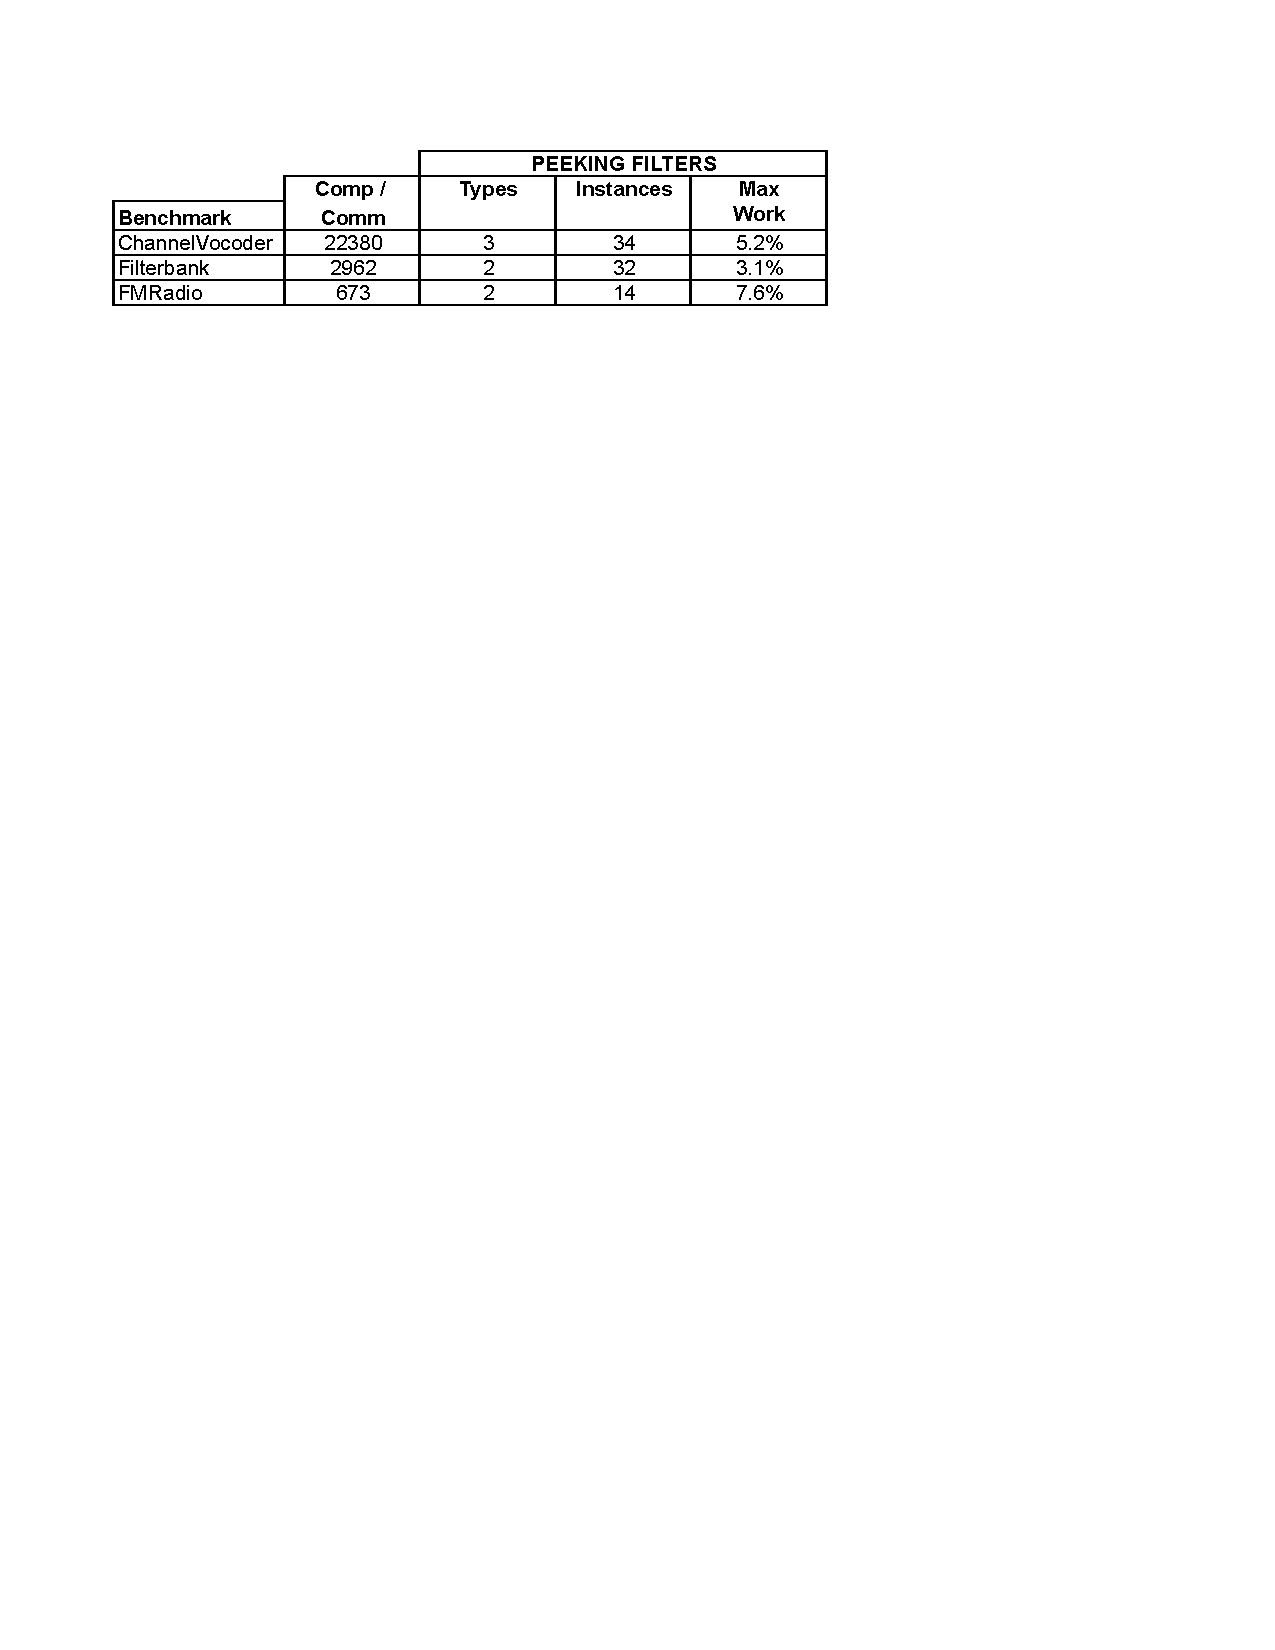
\includegraphics[width=3.3in]{figures/bench-char.pdf}}

\noindent ``Comp/Comm'' provides a static estimation of the
amount of computation to communication ratio by statically estimating the total
work of all the filters and dividing by the number items communicated
for the programmer-conceived graph's steady-state.  The remaining
statistics give the number of peeking filters types, number of peeking
filters instantiated at runtime, and a static estimation of the maximum
work in the single most loaded peeking filter.

We target 2 multicore architecture with different communication
mechanisms.  The Tilera Corporation's TILE64 Processor is a 64 core
system on a chip~\cite{tilera}.  Each core is an identical three-wide
VLIW. The code generated by the StreamIt
compiler for the TILE64 processor follows the remote store programming
(RSP) model~\cite{rsp10} in which each process has a private address
space, but each process can award remote processes write access to
their local memory. When a producer process has write access to a
consumer process's memory, the producer communicates directly with the
consumer via store instructions whose destination is an address in the
consumer's shared memory.  Communication is initiated by the producer,
and is fine-grained.  The consumer reads directly from it's local
memory (L2) when accessing input.

Our symmetric multiprocessor target is a 16-core architecture that is
comprised of four Intel Xeon E7350 multicore processors.  Each processor
is a 64-bit, quad-core with two dual-core dies.  Each die contains a 4
MB L2 cache shared across the two cores.  The front-side bus is clocked
at 1066 MHz.  We utilize the cache coherency mechanism of the
architecture for communication between cores. 

Through empirical experimentation on FMRadio, Filterbank, and
ChannelVocoder, we have settled on $T_{\mt{sharing}} =.10$ and
$T_{\mt{apply}} = 0.05$. These constants are the sweet stop for the two
architectures employed in the experimentation, being a good compromise
between buffer size and inter-core communication.

% \begin{figure*}[t]
% \centering
% \subfigure[]{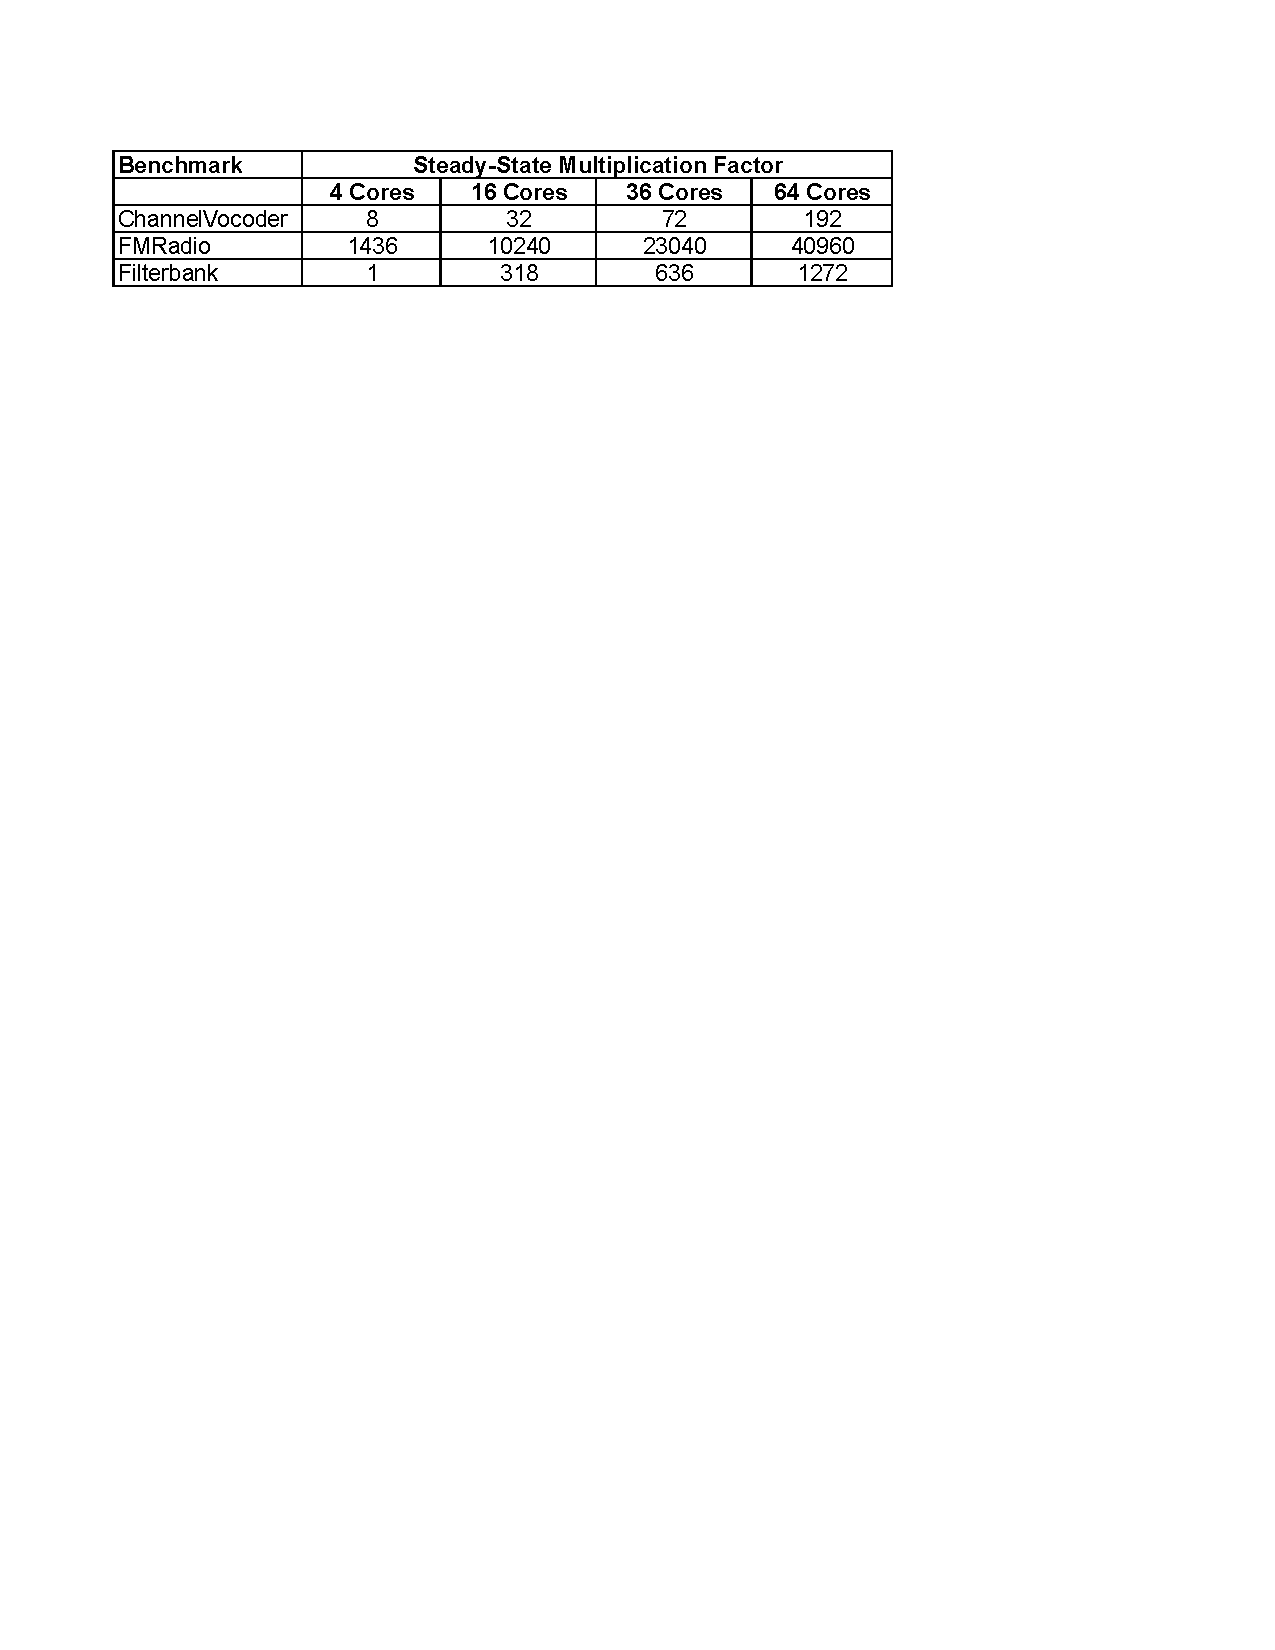
\includegraphics[width=3.7in]{figures/mult-table.pdf}} \\
% \subfigure[]{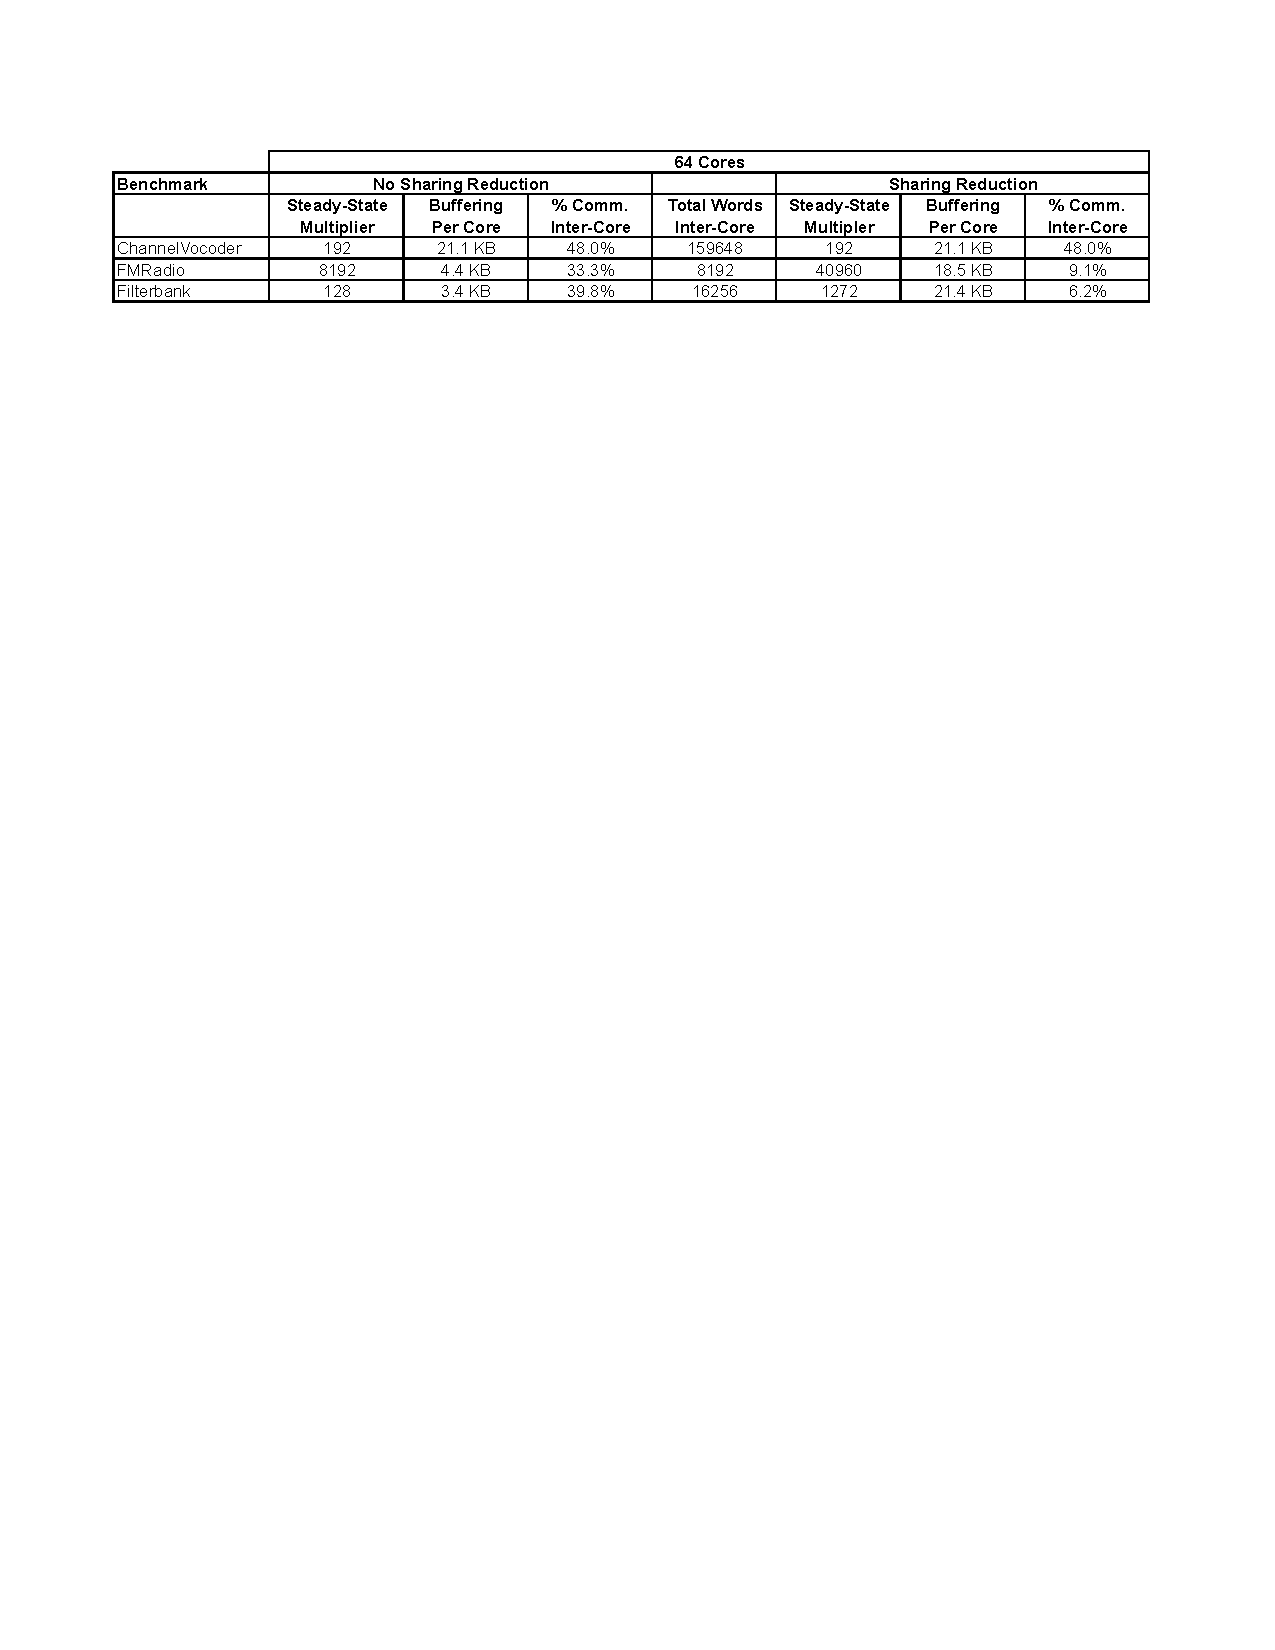
\includegraphics[width=6in]{figures/64-core-table.pdf}}
% \caption[Communication, multiplier and buffering statistics for
% benchmarks.]{
% Communication, multiplier and buffering characteristics for
% benchmarks: (a) gives the steady-state multipliers calculated for
% sharing reduction, (b) compares the steady-state with and without
% sharing reduction. 
% \label{fig:fission-table}}
% \end{figure*}

\begin{figure*}[t]
\centering
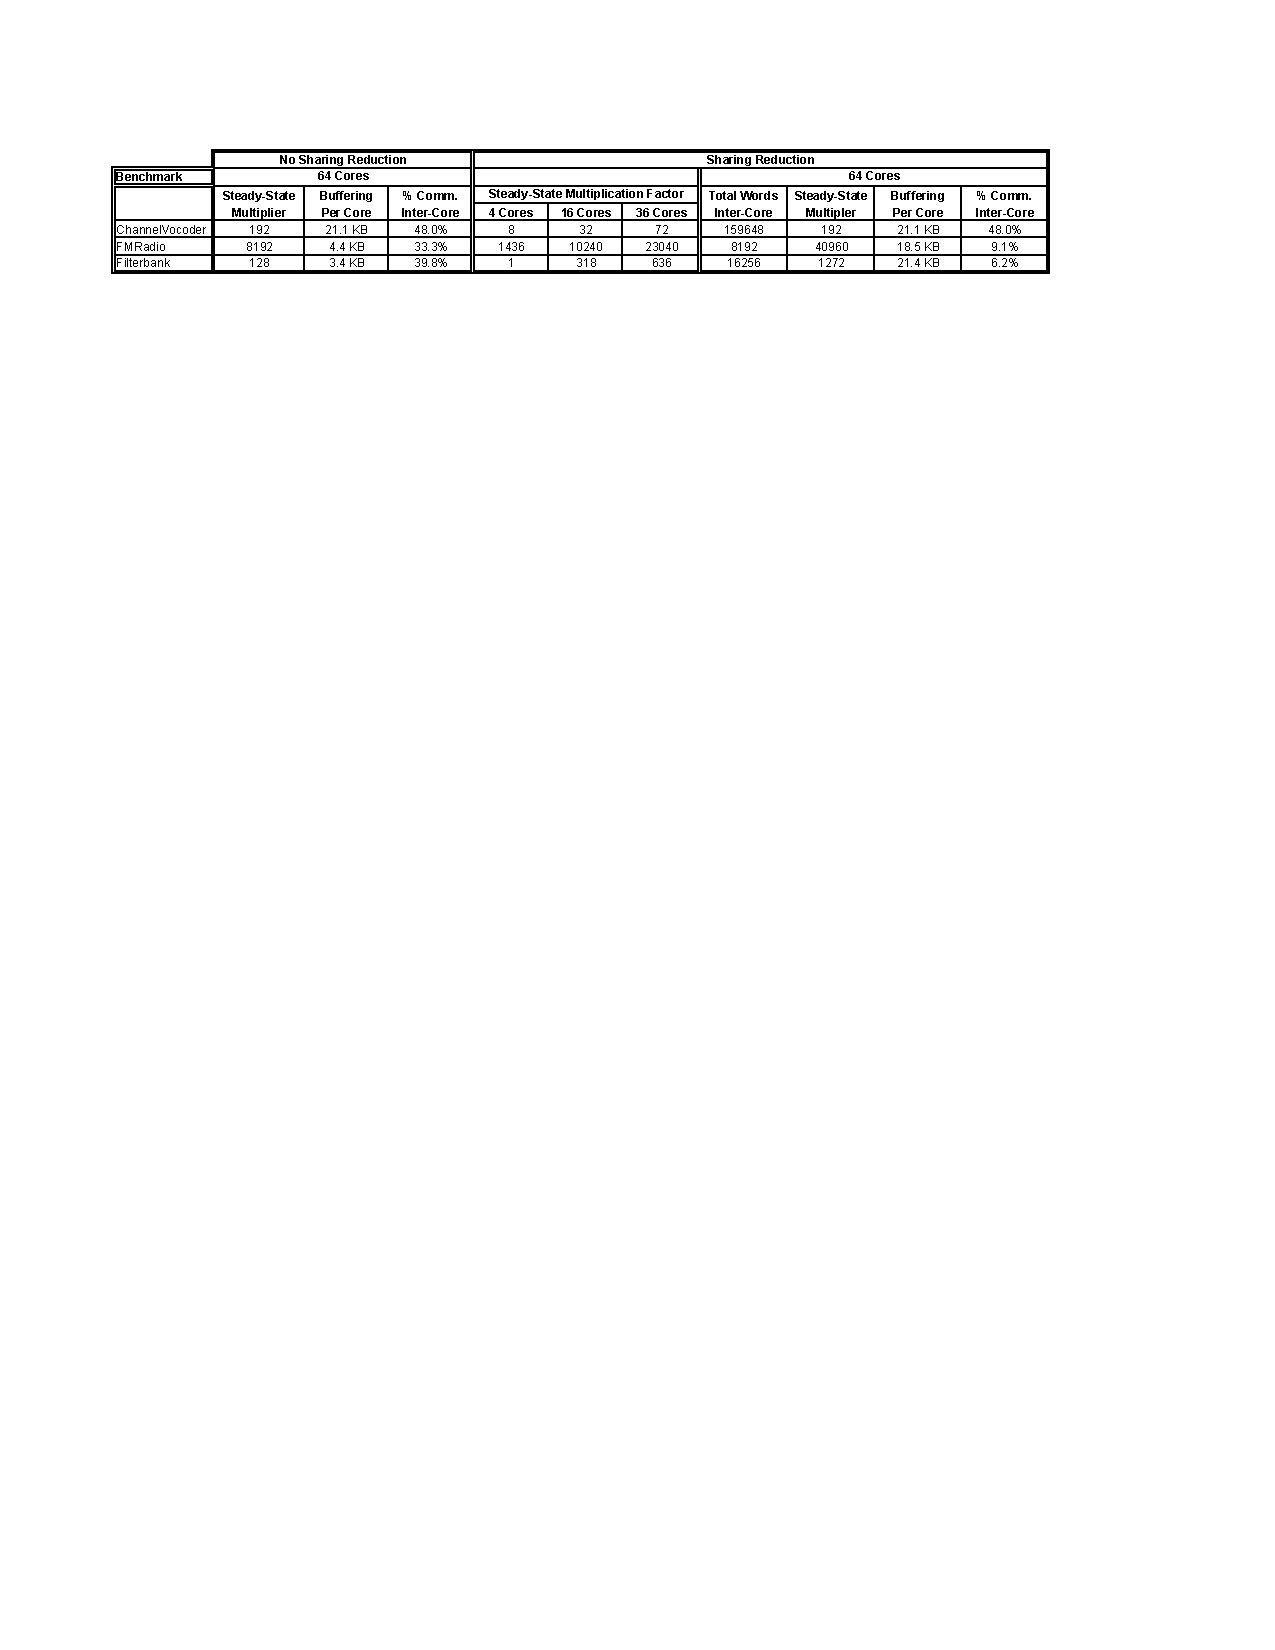
\includegraphics[width=6.1in]{figures/big-table.pdf}
\caption{\label{fig:big-table}  Steady-state multiplicity, buffering,
  and communication for fission with and without sharing reduction.}
\end{figure*}

% \begin{figure}[t]
% \centering
% 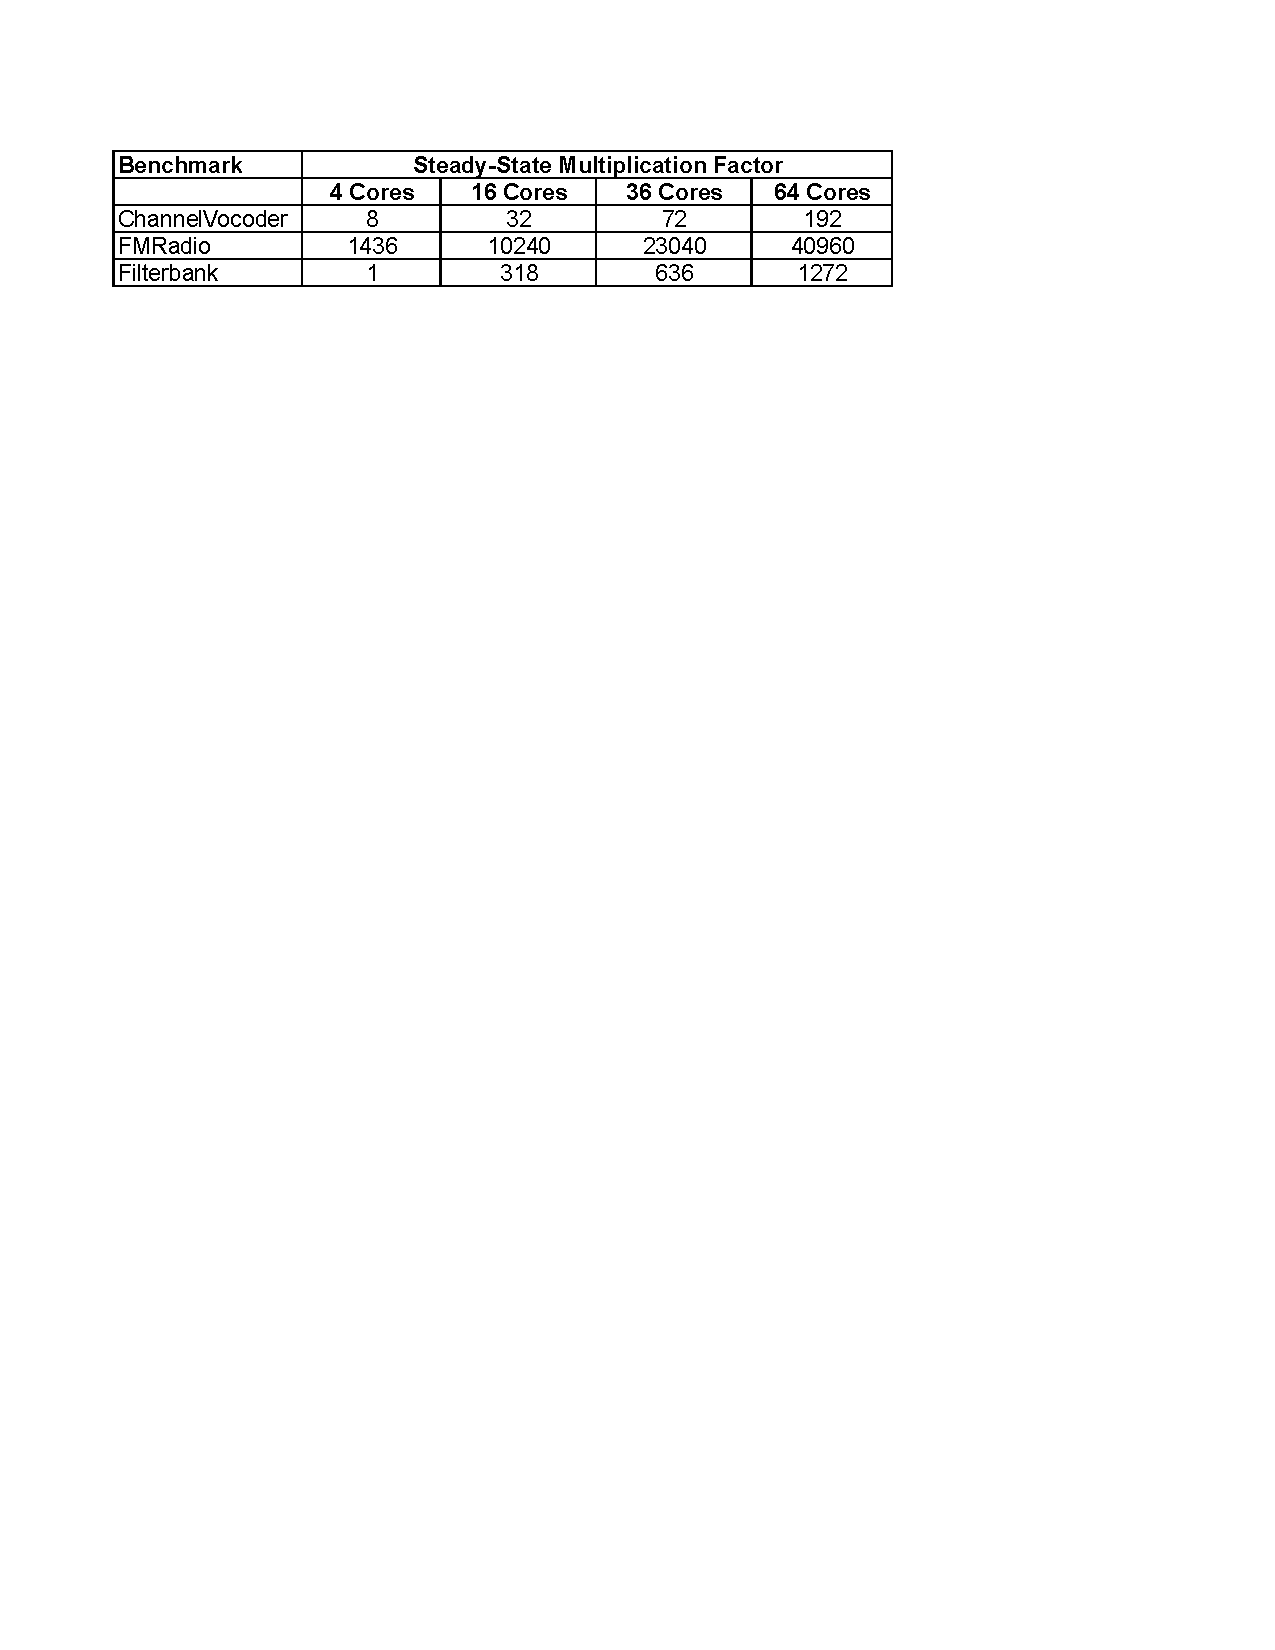
\includegraphics[width=3.3in]{figures/mult-table.pdf}
% \caption{\label{fig:mult-table}  The steady-state multipliers calculated for
% sharing reduction.}
% \end{figure}

% \begin{figure*}[t]
% \centering
% 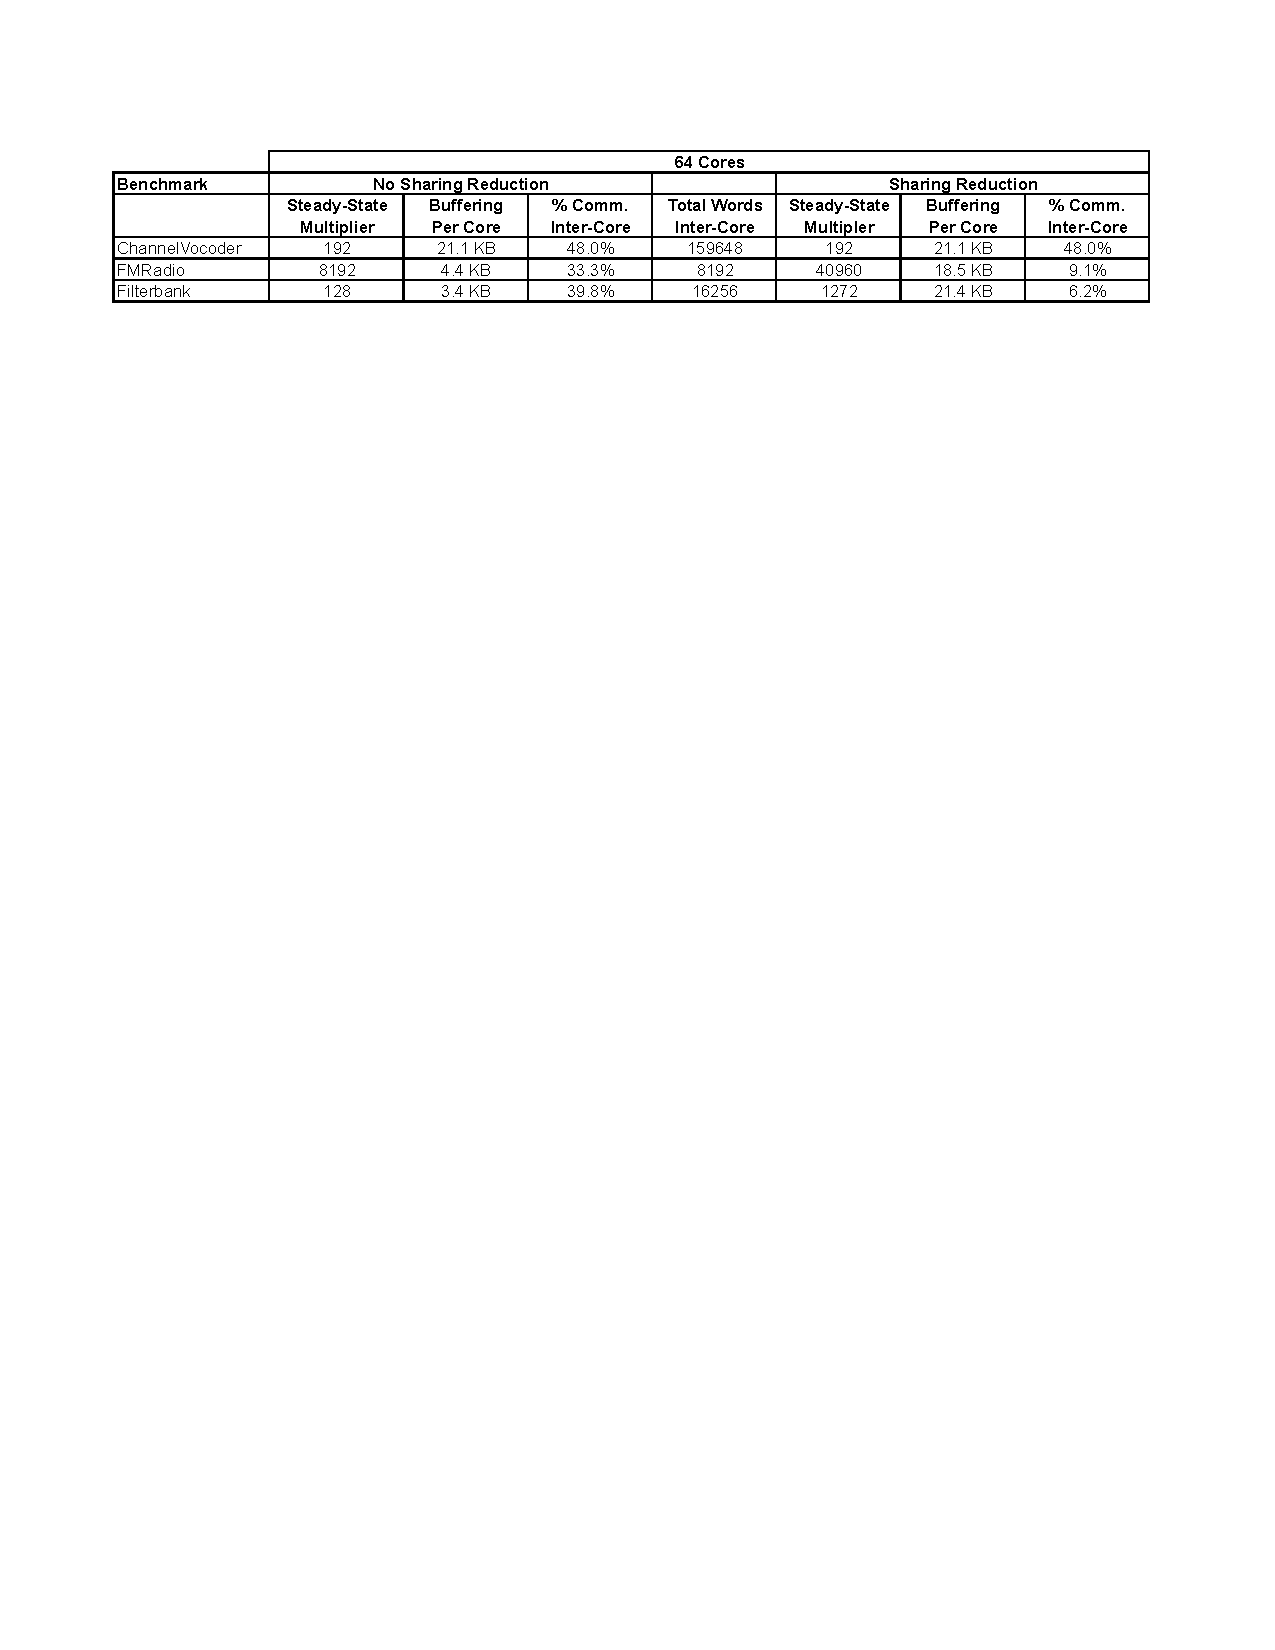
\includegraphics[width=6in]{figures/64-core-table.pdf}
% \caption{ Multiplier, buffering and communication for the steady-state with and without
% sharing reduction. 
% \label{fig:fission-table}}
% \end{figure*}

Figure~\ref{fig:big-table} compares the steady-state with and
without sharing reduction for a 64-core mapping, as well as gives the
constant $c$ calculated by sharing reduction for 4, 16, and 36.  The
factor is larger for FMRadio because one filter has $C(f) \gg o(S,
f)$.  The multiplication factor affects both latency and buffer sizes
adversely.  The application designer will have to decide if the
latency of these techniques can be borne given the application
criteria.  The total buffering requirement is increased when the
steady-state is increased.  However, since we are then fissing, the
buffer is divided amongst the fission products, and the {\it per-core}
buffering requirement is unaffected by the increase.  For example,
FMRadio, has a per-core 18 KB buffering requirement across all
configurations (4, 16, 36, and 64 cores).  This requirement fits in
the per-core L2 size of 64 KB for the Tile64.

 For ChannelVocoder,
sharing reduction has no effect because most of the peeking filters do
not satisfy $T_{\mt{apply}} = 0.05$ because of differing fission
factors between producers and consumers.  For the peeking filters that do,
the steady-state multiplier required for legal general fission for the
graph is enough to assure $T_{\mt{sharing}}$ is met.  Even though
sharing reduction has no effect for ChannelVocoder, general fission
avoids the 38\% of total items that were unnecessary duplicated by
DupDec.

For FMRadio and Filterbank, sharing reduction leads to significant
decreases in the percentage of total items communicated inter-core for
each steady-state.  The buffer requirement is increased an average of
5.2x for these benchmarks.  The total number of words communicated
inter-core during each steady-state is the same, with and without
sharing reduction.  However, the steady-state is greater in the
sharing reduction case, thus producing more outputs.

\begin{figure}[t]
\centering
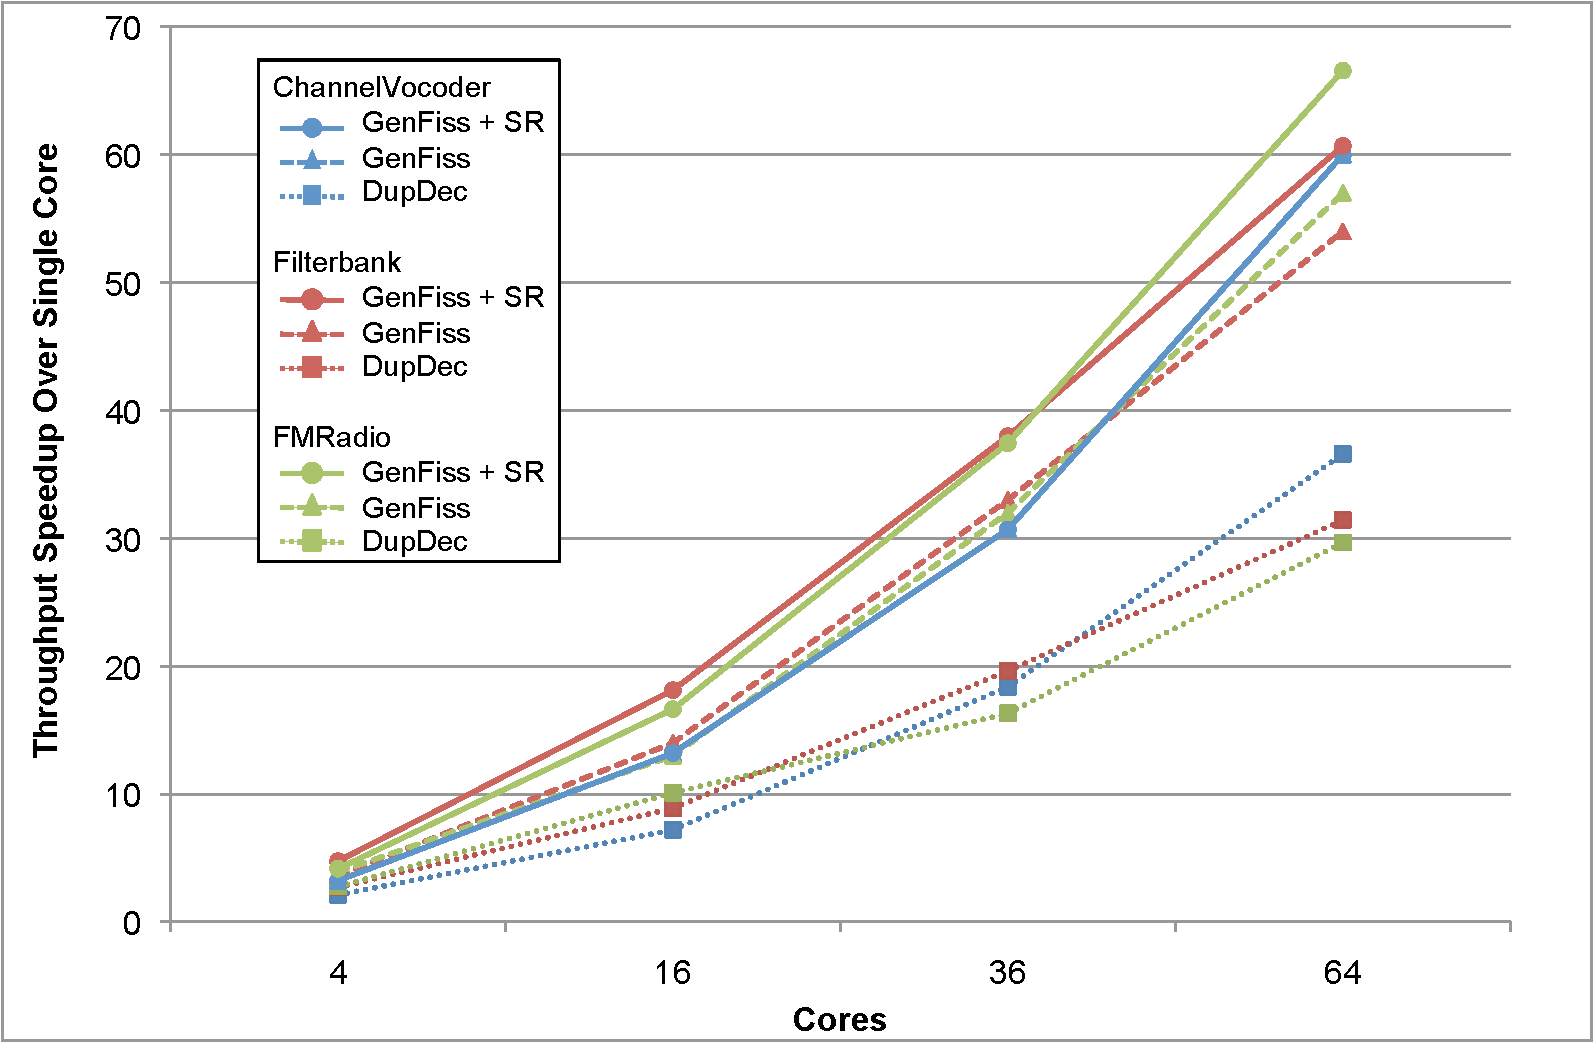
\includegraphics[width=3.3in]{figures/tilera-chart.pdf}
\caption[Comparing the fission techniques on the TILE64.]{
  Evaluation for DupDec versus general fission versus general fission with sharing reduction
  4, 16, 36, and 64 cores on the TILE64.  \label{fig:tilera-chart}}
\end{figure}

Figure~\ref{fig:tilera-chart} gives the performance results for the
Tilera TILE64 architecture.  We present results for DupDec, general
fission, and general fission with sharing reduction for 4, 16, 36, and
64 core configurations, with throughput normalized to single-core
throughput.  General fission with sharing reduction outperforms
DupDec by an average of 1.8x for the three benchmarks when targeting
64 cores. The average 64-core speedup over single core is 62.3x for the
general fission plus sharing reduction for these three benchmarks.

FMRadio experiences the most significant gain from general fission
plus sharing reduction over DupDec (67x versus 30x, respectively, for
64 cores).  FMRadio has the lowest computation to communication ratio
of the 3 benchmarks.  Furthermore, each filter of is fissed by the
number of cores targeted.  For 64 cores, each filter is fissed 64
ways.  DupDec must perform a global all-to-all communication involving
all 64 cores between each level of the graph!
 
ChannelVocoder achieves a 60x speedup for general fission over a
single core.  This is not perfectly linear because of the parallel
mapping; asymmetries exist between the extent of task parallelism and
the number of cores (see~\ref{mgordon-asplos06}).  The speedup over
DupDec (1.62x) is more modest because the width of many of the
fission applications is 3, so DupDec is duplicating input data to
groups of 3 filters.  Filterbank is similar, the width of fission is 4
for all filters when targeting 64 cores.

Sharing reduction is required to achieve scalable speedups for both
FMRadio and Filterbank.  For FMRadio, sharing reductions leads to a
17\% speedup increase for 64 cores.  This because sharing reduction
significantly reduces the number of remote write store instructions
required per output.  This affects FMRadio because of its low
computation to communication ratio.  Sharing reduction sees a 12\%
increase on Filterbank, as Filterbank has a larger computation to
communication ratio.

\begin{figure}[t]
\centering
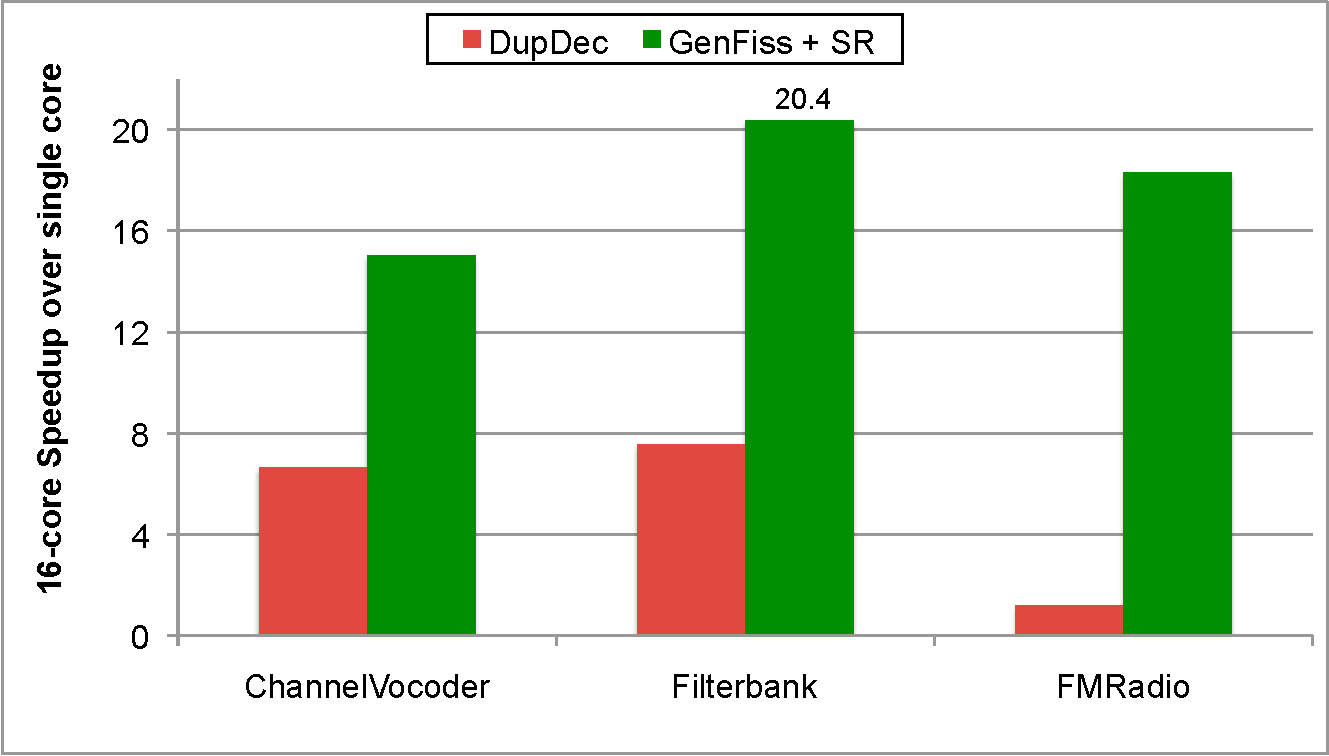
\includegraphics[width=3.3in]{figures/smp-chart.pdf}
\caption[Comparing the fission techniques on the 16-core SMP.]{
  Evaluation for DupDec versus general fission with sharing reduction
  for the 16-core SMP architecture.  \label{fig:smp-chart}}
\end{figure}

Our techniques enable scalable parallelization, with a mean speedup of
17x for our 3 benchmarks on the SMP.  Figure~\ref{fig:smp-chart} gives
the 16-core speedup comparison for DupDec versus general fission with
sharing reduction for our target SMP architecture.  The mean speedup
increase for general fission with sharing reduction over DupDec is
6.7x.  FMRadio again sees the largest speedup increase in the
comparison at 13.0x.  The reasons for this large speedup are similar
as given in the previous section.  However, the SMP communication
mechanism is not as efficient as the TILE64, thus general fission with
sharing reduction gives a greater speedup because reducing inter-core
communication has more impact.

\section{Related Work}
\label{sec:related}

% BILL

%Signal~\cite{Signal}, 
%Lucid~\cite{Lucid77}, and
%Occam~\cite{Occam}, and Sisal \cite{sisal}.
%Parallel Haskell~\cite{ph}
In addition to StreamIt, there are a number of stream-oriented
languages drawing from domains such as functional, dataflow, CSP and
synchronous programming~\cite{survey97}.  The Brook language is
architecture-independent and focusses on data
parallelism~\cite{brook04}.  Stream kernels are required to be
stateless, though there is special support for reducing streams to a
single value.  Stream\-C/Ker\-nel\-C is lower level than Brook;
kernels written in KernelC are stiched together in StreamC and mapped
to the data-parallel Imagine processor~\cite{imagine03ieee}.  SPUR
adopts a similar decomposition between ``microcode'' stream kernels
and skeleton programs to expose data parallelism~\cite{spur05samos}.
Cg exploits pipeline parallelism and data parallelism, though the
programmer must write algorithms to exactly match the two pipeline
stages of a graphics processor~\cite{cg03}.  Compared to these
languages, StreamIt places more emphasis on exposing task and pipeline
parallelism (all the languages expose data parallelim).
%and on sliding window operations (filters that peek).  
By adopting the synchronous dataflow model of execution~\cite{lee87},
StreamIt focusses on well-structured programs that can be aggressively
optimized.  The implicit infinite loop around programs is also a key
StreamIt characteristic that enables the transformations in this
paper.  Spidle is also a recent stream language that was influenced by
StreamIt~\cite{spidle03}.
%and Lucid Synchrone~\cite{Lucid-Synchrone}.
%Synchronous languages which
%target embedded applications include Esterel~\cite{Esterel},
%Lustre~\cite{Lustre}, and Additional

Liao et al. map Brook to multicore processors by leveraging the affine
partitioning model~\cite{liao06brook}.  While affine partitioning is a
powerful model for parameterized loop-based programs, in StreamIt we
simplify the problem by fully resolving the program structure at
compile time.  This allows us to schedule a single steady state using
flexible, non-affine techniques (e.g., simulated annealing) and to
repeat the found schedule for an indefinite period at runtime.
Gummaraju and Rosenblum map stream programs to a general-purpose
hyperthreaded processor~\cite{gummaraju05micro}.  Such techniques
could be integrated with our spatial partitioning to optimize per-core
performance.  Gu et al. expose data and pipeline parallelism in a
Java-like language and use a compiler analysis to efficiently extract
coarse-grained filter boundaries~\cite{du03sc}.  Ottoni et al. also
extract decoupled threads from sequential code, using hardware-based
software pipelining to distribute the resulting threads across
cores~\cite{ottoni05decoupled}.  By embedding pipeline-parallel
filters in the programming model, we focus on the mapping step.

%%%%%%%%%%%%%%%%%%%%%%%%%%%%%%%%%%%%%%%%%%%%%%%%%%%%%%%%%%%%%%%%%%%%%

Previous work in scheduling computation graphs to parallel targets has
focused on partitioning and scheduling techniques that exploit task
and pipeline parallelism~\cite{SDFSched, SDFSched2,may87communicating,
DAGSched, pipeline-sdf}.  Application of loop-conscious
transformations to coarse-grained dataflow graphs has been
investigated.  Unrolling (or ``unfolding'' in this domain) is employed
for synchronous dataflow (SDF) graphs to reduce the initiation
interval but they do not evaluate mappings to actual
architectures~\cite{unfolding,unfolding2}. Software pipelining
techniques have been applied to SDF graphs onto various embedded and
DSP targets~\cite{bakshi99,chatha-02}, but has required programmer
knowledge of both the application and the architecture. To our
knowledge, none of these systems automatically exploit the combination
of task, data, and pipeline parallelism.  Furthermore, these systems
do not provide a robust end-to-end path for application
parallelization from a high-level, portable programming language.

%% Previous work on instruction-level software pipelining has focused
%% mostly on scheduling machine instructions in a loop via modulo
%% scheduling~\cite{rau81,lam-softpipe}.  The algorithms devised must
%% account for tight resource constraints and complex instruction
%% dependences. Our software-pipelining problem is much less constrained,
%% enabling us to employ a simple greedy heuristic.  

%% Furthermore, a traditional modulo scheduling algorithm is not needed
%% because we have an implicit loop barrier at the end of each
%% steady-state.  ILP compilers for clustered VLIW
%% architectures~\cite{Bulldog,Multiflow,lee98spacetime,qian02} must
%% partition instructions and assign them to clusters as part of the
%% instruction scheduling. Clustering is analogous to our application of
%% filter fusion in our software pipelining algorithm.

\section{Conclusion}
\label{sec:conclusion}

In this paper, we describe the StreamIt compiler for the Raw
architecture.  The stream graph of a StreamIt program exposes the data
communication pattern to the compiler while the lack of global
synchronization frees the compiler to radically reoganize the program
for efficient execution on the underline architecture. The StreamIt
compiler demonstrates the power of this flexibility by totally
reoganizing large programs for better load balance. We were able to
map many of programs on to the Raw processor and obtain good
performance.

We introduce a collection of optimizations, vertical and horizontal
filter fusion, vertical and horizontal filter fission and filter
reordering transformations, that can be used to restructure stream
graphs.  We show that by applying these transformations we can map a
high-level stream program, written to reflect the composition of the
application, onto Raw and achieve good processor utilization and load
balance, leading to a factor of three speedup on two applications.

Unlike all previous streaming languages, the structured streams of
StreamIt makes it possible for us to approach the optimization and
parallelization problems in a very systermatic manner. It enables us
to define multiple optimizations -- targetting different constructs
and requirements -- and to compose them them in a hirearchical manner.

The ability to do global transformations across multiple filters, that
may have originated from very different parts of the application,
makes it possible for the compiler to find optimization opportunities
that may ellude even an experience programmer.  Such capabilities
enables the programmers to write protable streaming applications and
map them efficiently onto any given architecture. This has the
potential of creating a programming standard for emerging
communication exposed architectures.  The StreamIt compiler takes a
fist step towards this goal.


\section{Acknowledgements}

We are very grateful to Anant Agarwal, Mike Taylor, Davind Wentzlaff,
Walter Lee, Matt Frank, and the rest of the Raw group for their
development of the Raw infrastructure and wholeharted support of this
project.  This work is supported in part by a grant from DARPA (PCA
F29601-04-2-0166), an award from NSF (CISE EIA-0071841), and a
fellowship from the Singapore-MIT Alliance.


% Bibliography -- whee!
{\small
  \bibliographystyle{abbrv}
  \bibliography{references}
}

%\appendix
\clearpage
%%\section{StreamGraphs}

% This appendix has all of the stream graphs for the 
% benchmark programs used in the paper

\begin{figure*}[t]
  \center
  %{\bf Appendix A: Benchmark Stream Graphs} \\ ~ \\ ~ \\
  \begin{tabular}{ccc}
    \begin{minipage}{3in}
      \center
      \begin{tabular}{cc}
	\begin{minipage}{1.2in}
	  \center
	  \epsfxsize=1.0in
	  \epsfbox{streamgraphs/fir.ps} 
	\end{minipage} &
	\begin{minipage}{1.2in}
	  \center
	  \epsfxsize=1.0in
	  \epsfbox{streamgraphs/sample.ps}
	\end{minipage}\\
      \end{tabular}
    \end{minipage} & ~\hspace{0.5in} & 
    \begin{minipage}{3in}
      \center
      \epsfysize=1.8in
      \epsfbox{streamgraphs/target.ps} 
    \end{minipage}  
    \\
    \begin{tabular}{cc}
      \begin{minipage}{1.2in}
	\center
	{\bf a) FIR} 
      \end{minipage} &
      \begin{minipage}{1.2in}
	\center
	{\bf b) RateConvert} 
      \end{minipage}\\
    \end{tabular} & &
    \begin{minipage}{3in}
      \center
      {\bf c) TargetDetect}
    \end{minipage}
    \\~\\

    \multicolumn{3}{c}{
      \begin{tabular}{cc}
	\begin{minipage}{4in}
	  \center
	  \epsfysize=1.8in
	  \epsfbox{streamgraphs/fm.ps}
	\end{minipage} &
	\begin{minipage}{2in}
	  \center
	  \epsfysize=1.8in
	  \epsfbox{streamgraphs/vocoder.ps}
	\end{minipage} \\
      {\bf d) FM} & {\bf e) Vocoder} \\
      \end{tabular}
    }
    
    \\~\\

    \multicolumn{3}{c}{
      \begin{tabular}{cc}
	\begin{minipage}{5in}
	  \center
	  \epsfxsize=5.0in
	  \epsfbox{streamgraphs/bf.ps}
		  {\bf f) Radar}
	\end{minipage} &
	\begin{minipage}{1in}
	  \center
	  \begin{tabular}{c}
	    \epsfxsize=0.5in
	    \epsfbox{streamgraphs/oversampler.ps} \\
            {\bf g) Oversample} \\
	  \end{tabular}
	\end{minipage} \\
      \end{tabular}
    }
  
    \\~\\

    \begin{minipage}{2.5in}
      \center
      \epsfysize=2.5in
      \epsfbox{streamgraphs/onebit.ps}
    \end{minipage} &  &
    \begin{minipage}{3in}
      \center
      \epsfysize=2.5in
      \epsfbox{streamgraphs/fb.ps}
	
    \end{minipage}
    \\
    {\bf h) OneBit}  & & 
    {\bf i) FilterBank}
    \\
 
    
  \end{tabular}
  \caption{Benchmark Stream Graphs.}
  \label{fig:streamgraphs}
\end{figure*}

\clearpage
%{\bf Appendix C:  Frequency Replacement Scaling} \\ ~ \\ ~ \\



\begin{figure*}[t]
\center
\begin{minipage}{3.4 in}
\center
\epsfxsize=2.2in
\epsfbox{images/frequency-win-theory.eps} \\
{\bf (a): Theoretical}
\end{minipage} 
\begin{minipage}{3.4 in}
\center
\epsfxsize=2.2in
\epsfbox{images/frequency-win-empirical.eps} \\
{\bf (b): Empirical}
\end{minipage}
\caption{Plots showing the theoretical and empirical multiplication reduction factor as a function of the size of the FIR ($M$) and the number of outputs produced per calculation ($N$). The dark regions denote an increase in the required number of multiplications and the light regions a reduction.}
\label{fig:frequency-win}
\end{figure*}

Frequency replacement is an effective optimization because the asymptotic bounds for 
frequency domain computation is lower than the bound for the time domain computation. 
We determined empirically the point at which frequency replacement improves performance.
  
Direct convolution requires $O(MN)$ multiplies. 
The FFT requires $O(N+2(M-1))lg(N+2(M-1))$ multiplications for both the
conversion to and from the frequency domain, and multiplying two $N+2(M-1)$
vectors in the frequency domain requires $O(N+2(M-1))$ multiplications. 
Direct convolution produces $N$ outputs per iteration and the frequency implementation 
produces $N+M-1$ outputs every iteration. 
We define the ``multiplication reduction factor''
to be the number of multiplies required per output using convolution divided by the 
the number of multiplies per output using the frequency transformation.

Figure~\ref{fig:frequency-win}~(a) shows a plot of the theoretical multiplication reduction factor
and Figure~\ref{fig:frequency-win}~(b) shows the same reduction factor measured empirically. 
The roughness in both the theoretical results and the data is due to the fact that
our FFT algorithm requires $N+2(M-1)$ to be a power of two, and the compiler
automatically adjusts $N$ upward to satisfy this requirement. The theoretical 
reduction numbers account for the fact that our implementation requires four 
floating point multiplication operations to perform a complex valued multiply 
in the frequency domain.

Based on the above analysis, our current compiler applies the frequency replacement
transformation on FIR filters that have length $90$ or greater. The target output
rate, $N$, is automatically set to be twice the FIR length.

\end{document}